\documentclass[12pt]{amsart}
\usepackage[shortlabels]{enumitem}
\usepackage{fullpage,graphicx,psfrag,amsmath,amsfonts,verbatim, amssymb, caption, subcaption,booktabs, hyperref}
\newtheorem{theorem}{Theorem}[section]
\newtheorem{prop}{Proposition}[section]
\newtheorem{corollary}{Corollary}[section]
\newtheorem{lemma}[theorem]{Lemma}
\newtheorem{problem}[theorem]{Problem}
\newtheorem{conj}[theorem]{Conjecture}

%%% DEF 
\newcommand{\Z}{\mathbb{Z}}
\newcommand{\R}{\mathbb{R}}

\title{Dynamic dimensional reduction in the Abelian sandpile}
\author{Ahmed Bou-Rabee}
\address{Ahmed Bou-Rabee\\
  Department of Statistics\\
  University of Chicago\\
  5747 S. Ellis Avenue\\
  Chicago, IL 60637, USA}
  
  \subjclass[2010]{82C27, 37B15, 39A12}
\keywords{Abelian sandpile, dimensional reduction, parabolic least action principle, discrete regularity.}
  
  
\begin{document}
	
	\begin{abstract}
		We prove the dimensional reduction conjecture of Fey, Levine, and Peres (2010) on the hypercube. 
		The proof shows that dimensional reduction, symmetry, and regularity of the Abelian sandpile persist during the parallel toppling process. This stronger result verifies empirical observations first documented by Liu, Kaplan, and Gray (1990).  %(Geometry and dynamics of deterministic sandpiles). 
	\end{abstract}
	\maketitle
	
	\section{Introduction}
	
	\subsection{Overview} 
	Let $\mathcal{C}_N^{(d)}$ be a hypercube of side length $N$ centered at the origin in the $d$-dimensional integer lattice $\Z^d$.  A {\it sandpile} is a function $s: \mathcal{C}_N^{(d)} \to \Z$. Start with $2d$ chips in the hypercube,  $s = s_0^{(d)} \equiv 2d$, then iterate the following rule: every site with at least $2d$ chips on it becomes {\it unstable} 
	and {\it topples} in {\it parallel}, simultaneously giving one chip to each of its $2d$ neighbors. If a boundary site topples, it loses chips over the edge. Eventually every site is stable and the process stops, yielding a sequence of sandpiles over time $\{s_t^{(d)}\}_{t \geq 0}$ \cite{bak1987self, dhar1990self, holroyd2008chip,levine2010sandpile,levine2017laplacian,jarai2018sandpile, klivans2018mathematics}.
	
	Simulations suggest an exact relationship between these sandpiles across size $N$, time $t$, and dimension $d$ --- see Figures \ref{fig:2d} and \ref{fig:3d}. 
	Specifically, it appears that smaller sandpiles are embedded in larger sandpiles of the same dimension at certain times. Moreover, 
	central cross sections of $d$-dimensional sandpiles coincide almost exactly with $(d-1)$-dimensional sandpiles for all time.  
	
	In this article, we provide a rigorous proof of these observations, {\it self-similarity} and {\it dimensional reduction}, 
	via a simultaneous induction on all parameters: size, time, and dimension. Along the way, we develop new techniques for analyzing the parallel toppling process which may be of independent interest.  %The proof strategy (and result) is inspired by  elliptic PDE regularity but the paper is entirely self-contained and the arguments are discrete. 

	
	\begin{figure}[!hb]
		\begin{centering}
			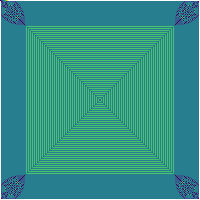
\includegraphics[width=0.22\textwidth]{Figures/2D_dynamic_N200_25.png}
			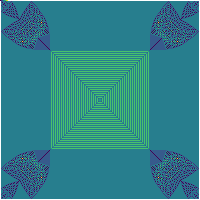
\includegraphics[width=0.22\textwidth]{Figures/2D_dynamic_N200_50.png} 
			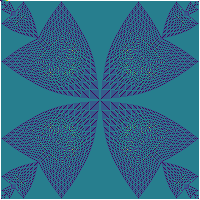
\includegraphics[width=0.22\textwidth]{Figures/2D_dynamic_N200_100.png}
			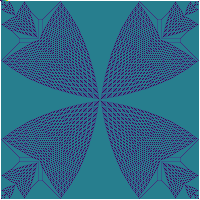
\includegraphics[width=0.22\textwidth]{Figures/2D_dynamic_N200_200.png}
		\end{centering}
		\caption{ $s_t^{(2)}$ for $t = (25)^2, (50)^2, (100)^2, \infty$,  where $N=200$ and $s_0 \equiv 4$. Sites with $0,\ldots,7$ chips 
			are represented by different colors.  \label{fig:2d} }
	\end{figure}
	
	\begin{figure}[tbp] 
		\begin{centering}
			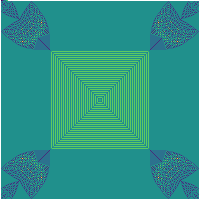
\includegraphics[width=.22\textwidth]{Figures/3D_dynamic_N200_k50_offSet0.png}
			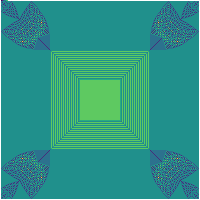
\includegraphics[width=.22\textwidth]{Figures/3D_dynamic_N200_k50_offSet20.png}
			
\includegraphics[width=.22\textwidth]{Figures/3D_dynamic_N200_k50_offSet40.png}
			
\includegraphics[width=.22\textwidth]{Figures/3D_dynamic_N200_k50_offSet60.png}
		\end{centering}
		\setlength{\belowcaptionskip}{-20pt} 
		\caption{ $s_t^{(3)}(\cdot, \cdot, \mbox{offset})$ for 
			$\mbox{offset} = 0, 20, 40, 60$, where $t = (50)^2$, $N=200$, and $s_0 \equiv 6$.  Sites with $0,\ldots,11$ chips are represented by different colors and `offset' 
			is distance to the center of $\mathcal{C}_N^{(3)}$. \label{fig:3d} }
	\end{figure}
	Dimensional reduction in sandpiles has been known experimentally since at least the work of Liu, Kaplan, and Gray in 1990 \cite{liu1990geometry}.
	In 2010, Fey, Levine, and Peres formulated an approximate dimensional reduction conjecture in the context of the single-source sandpile \cite{fey2010growth} --- this was later highlighted in a survey by Levine and Propp \cite{levine2010sandpile}.  Soon after, Pegden and Smart, in a breakthrough, used the theory of viscosity solutions to show that the large-scale patterns which appear in sandpiles can be described by a limiting {\it sandpile PDE} \cite{pegden2013convergence}. This led to a series of works, joint with Levine, which provide a remarkable understanding of sandpiles on $\Z^2$ \cite{levine2017apollonian, levine2016apollonian, pegden2020stability}. 
	
	The structure of the sandpile PDE reveals that on torus-like domains one can construct limit 
sandpiles in $\R^d$ from those in $\R^{d-1}$.  This is also possible for certain random sandpiles \cite{bou2021convergence}. However, it has remained completely open to prove (or disprove) dimensional reduction for any natural example, on either the lattice or the continuum, till now. 

	Our proof in this paper leverages discrete techniques to establish dimensional reduction on the hypercube when $s_0 \equiv 2d$. The main insight is recognizing that the parallel toppling process together with strong induction can be used to control the sandpile as it stabilizes.  We identify a delicate interplay between the initial condition and the symmetry of the hypercube which forces the `flow' of parallel toppling to preserve dimensional reduction. In fact, we do not know how to prove dimensional reduction for only the terminal sandpile. Our proof involves no technology from viscosity solutions nor knowledge of the sandpile PDE.
	
	A key step in the proof is the application of certain discrete derivative bounds  --- Corollary \ref{cor:derivative_bound} and Lemma \ref{topple_limit} below. The strength of these bounds deteriorates as the initial condition grows and it is only when $s_0 \equiv 2d$ that they are strong enough to ensure dimensional reduction. 
	
	This dependence on the initial condition provides some explanation for what occurs in the single-source version. Fey-Levine-Peres conjectured 
	that when 	the initial condition is $(2 d- 2 ) + n \delta_0$  dimensional reduction occurs after carving out a region near the origin. This is likely because 
	our derivative bound (which, in the single-source version, has a flipped dependence on the constant background) does not hold near the origin, but only holds away from it.  Proving this remains open, but we believe the methods in this paper extend to 
	this and other initial data. 
	
	In fact, the result in this paper appears to be a special case of a more general one which we cannot yet prove: dimensional reduction occurs for any uniform initial condition 
	in high enough dimensions. Specifically, for integer $k \geq 0$, when $s_0 \equiv 2d + k$, above a critical dimension, $d > d_0 := k+1$, exact dimensional reduction, modulo $(d_0-1)$-dimensional defects, appears to persist throughout the parallel toppling process. We show that when $d = d_0$, dimensional reduction fails to occur, providing one explanation for why $(d_0-1)$-dimensional defects appear --- see Table \ref{tab:strong_dim1}. 
	

	
	\subsection{Main Result}
	Our proof begins with the {\it odometer} $v_t$, which encodes the number of topples at each site over time. Let $v_0 : \mathcal{C}_N^{(d)} \to \mathbb{Z}^+$ be the initial odometer $v_0 \equiv 0$; then, recursively, 
	\begin{align}
	v_{t+1} &= v_{t} +  1\{ s_{t} \geq 2 d \}, \\
	s_{t+1} &= s_{t} + \Delta ( v_{t+1} - v_{t} ) ,
	\end{align}
	where $\Delta$ is the graph Laplacian on $\mathcal{C}_N^{(d)}$ with dissipating boundary conditions.  Dependence on $d$ and $N$ is indicated by writing $v_t^{(d,N)}$ and $s_t^{(d,N)}$. %When dependence is clear from the context, the superscripts are dropped. 
	
	
	We prove dimensional reduction and self-similarity of sandpiles
	via an analysis of the parallel toppling odometers.  It will be more convenient to state the result after making a symmetry reduction. 
	 Let $\operatorname{Aut}_{\mathcal{C}_d}$ denote the group of symmetries of the $d$-dimensional hypercube and let it act on $\Z^d$ by matrix-vector multiplication.
	 The definitions imply that parallel toppling preserves the symmetries of the hypercube: 	$v_t^{(d,N)}(\mathbf{x}) = v_t^{(d,N)}( \sigma \mathbf{x})$ for all $t \geq 1$, $\mathbf{x} \in \mathcal{C}_N^{(d)}$, and $ \sigma \in \operatorname{Aut}_{\mathcal{C}_d}$ (we give a simple proof in Section \ref{subsec:symmetry} below).
	 Hence the odometer and sandpile are fully determined by their restrictions to
	a fundamental domain of the hypercube --- we choose a particular one in the statement of the theorem. 
	
	
	\begin{theorem}\label{the_theorem}
		Let $N \geq 1$, $d \geq 2$, and $M = \lceil N/2 \rceil$. Denote the fundamental domain of $\mathcal{C}_N^{(d)}$
		consisting of sorted coordinates in decreasing order by $\mathcal{S}^{(d)}_M := \{ (x_1, \ldots, x_d): M \geq x_1 \geq \cdots \geq x_d \geq 1 \}$.
		
		\begin{enumerate}
			\item{Dimensional reduction:} for all $t \geq 1$ and $\mathbf{x}_{d-1} \in \mathcal{S}_M^{(d-1)}$
			\begin{equation*}
			v_t^{(d, N)}(\mathbf{x}_{d-1}, 1) =  v_t^{(d-1, N)}(\mathbf{x}_{d-1})
			\end{equation*}
			and for $\mathbf{x}_{d-1} \geq 2$ 
			\begin{equation*}
			v_{\infty}^{(d,N)}(\mathbf{x}_{d-1}, 2) =  v_{\infty}^{(d-1,N)}(\mathbf{x}_{d-1}).
			\end{equation*}
			\item{Self-similarity:} for all $j < M$, $t \leq \tau_j$, and $\mathbf{x} \in \mathcal{S}_M^{(d)}$ with $\mathbf{x} > M-j$
			\begin{equation*}
			v_t^{(d, N)}(\mathbf{x}) = v_t^{(d, 2 j)}(\mathbf{x}-(M-j)),
			\end{equation*}
			where 
			\begin{equation*}
			\tau_{j} := \min\{ t \geq 1: v_t^{(d,2 j)}(\mathbf{x}) \geq j
                \mbox{ for some $\mathbf{x}\in\partial\mathcal{C}^{(d)}_{2j}$}\},
                \qquad(\min\varnothing:=+\infty).
			\end{equation*}
			and $\partial \mathcal{C}^{(d)}_i := \{ \mathbf{x} \in \mathcal{C}^{(d)}_i : \mbox{there is $\mathbf{y} \not \in \mathcal{C}^{(d)}_i$ with $|\mathbf{y}-\mathbf{x|} = 1$}\}$ denotes the inner boundary of the cube.
			%Moreover, the growing boundaries reflect: for $\mathbf{x}_{d-1} > M-j$, 
			%\begin{equation} \label{eq:reflecting_boundaryD}
			%    v_t^{(d,M)}(\mathbf{x}_{d-1}, (M-j)) = v_t^{(d,M)}(\mathbf{x}_{d-1}, (M-j)+1)
			%\end{equation}
			
		\end{enumerate}
		
		
		
	\end{theorem} 

	Both of these results immediately translate to the sandpile. 
	\begin{corollary}\label{sandpile_corollary} 
		% For each integer $k \geq 0$, the following hold for all $d \geq d_0 := (k + 2)$.
	
		The results in Theorem \ref{the_theorem}, using the same notation, extend to the sequence of sandpiles. 	
		%The following holds, in the same setting as 
		\begin{enumerate}
			\item{Dimensional reduction:} for all $\mathbf{x}_{d-1} \in \mathcal{S}_M^{(d-1)}$ with $\mathbf{x}_{d-1} \geq 2$
			\[
			s_{\infty}^{(d,N)}(\mathbf{x}_{d-1},1)  = s_{\infty}^{(d-1,N)}(\mathbf{x}_{d-1})+2.
			\]
			\item{Self-similarity:} for all $j < M$, $t \leq \tau_j$, and $\mathbf{x} \in \mathcal{S}_M^{(d)}$ with $\mathbf{x} > M-j+1$
			\[
			s_t^{(d,N)}(\mathbf{x}) = s_t^{(d,2 j)}(\mathbf{x}-(M-j)).
			\]
			\end{enumerate}

	\end{corollary}
	
	The first part of Theorem \ref{the_theorem} states that the parallel toppling odometer restricted to a center slice of a $d$-dimensional hypercube coincides 
	with the $(d-1)$-dimensional parallel toppling odometer for all time.  Dimensional reduction holds for the final odometer off the center, implying dimensional reduction 
	on the center for the final, stable sandpile. 
	
	The second part of the theorem relates the parallel toppling odometers for different sized cubes: 
	the odometer for the size $N$ cube contains the size $2 j$ cube odometer up until the first time a boundary site exceeds $j$ topples. These automatically imply, after shrinking the domains by one, the same for the sequence of sandpiles.
	
	
	
	
	
	\begin{table}      
		\begin{tabular}{cccccc}
			\toprule
			$k$ & 0  & 1 & 2 & 3 & 4 \\
			\midrule
			$s_{\infty}^{(2)}(\cdot, \cdot)$ & 
\includegraphics{figs/offsets_0/k0_d2_kk5_.png}  & 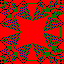
\includegraphics{figs/offsets_0/k1_d2_kk5_.png} & 
\includegraphics{figs/offsets_0/k2_d2_kk5_.png}   & 
\includegraphics{figs/offsets_0/k3_d2_kk5_.png}  &  
\includegraphics{figs/offsets_0/k4_d2_kk5_.png} \\
			$s_{\infty}^{(3)}(\cdot, \cdot,1)$ & 
\includegraphics{figs/offsets_0/k0_d3_kk5_.png}  & 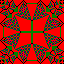
\includegraphics{figs/offsets_0/k1_d3_kk5_.png} & 
\includegraphics{figs/offsets_0/k2_d3_kk5_.png}   & 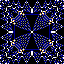
\includegraphics{figs/offsets_0/k3_d3_kk5_.png}  &  
\includegraphics{figs/offsets_0/k4_d3_kk5_.png} \\
			$s_{\infty}^{(4)}(\cdot, \cdot,1,1)$ & 
\includegraphics{figs/offsets_0/k0_d4_kk5_.png}  & 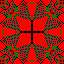
\includegraphics{figs/offsets_0/k1_d4_kk5_.png} & 
\includegraphics{figs/offsets_0/k2_d4_kk5_.png}   & 
\includegraphics{figs/offsets_0/k3_d4_kk5_.png}  &  
\includegraphics{figs/offsets_0/k4_d4_kk5_.png} \\
			$s_{\infty}^{(5)}(\cdot, \cdot,1,1,1)$ & 
\includegraphics{figs/offsets_0/k0_d5_kk5_.png}  & 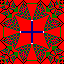
\includegraphics{figs/offsets_0/k1_d5_kk5_.png} & 
\includegraphics{figs/offsets_0/k2_d5_kk5_.png}   & 
\includegraphics{figs/offsets_0/k3_d5_kk5_.png}   &  
\includegraphics{figs/offsets_0/k4_d5_kk5_.png} \\
			$s_{\infty}^{(6)}(\cdot, \cdot,1,1,1,1)$ & 
\includegraphics{figs/offsets_0/k0_d6_kk5_.png}  & 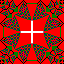
\includegraphics{figs/offsets_0/k1_d6_kk5_.png} & 
\includegraphics{figs/offsets_0/k2_d6_kk5_.png}   & 
\includegraphics{figs/offsets_0/k3_d6_kk5_.png}   &  
\includegraphics{figs/offsets_0/k4_d6_kk5_.png} \\
			\bottomrule
		\end{tabular}
		\caption{Center slices of terminal sandpile configurations for $s_0 \equiv 2 d + k$ and $N = 64$. Site colors are normalized by column so that in dimension $d$ a site with $z$ chips has the same color as a site with $(z-2)$ chips in dimension $(d-1)$.}
		\label{tab:strong_dim1}
	\end{table}

	As mentioned previously, we expect Theorem \ref{the_theorem} to be a special case of a more general result. 
	In Section \ref{sec:base_case} we show that dimensional reduction does not occur when $s_0 \equiv 2 d + (d-1)$ 
	 in all dimensions $d \geq 2$ when $N=2$. We also provide an explicit description of the parallel toppling odometer 
	when $s_0 \equiv 2 d + (d-1)$ and $N=4$ for all $d \geq 1$. This explicit form suggests that the proof template in this paper 
	may help with the following. 
	
	\begin{problem} \label{prob:true_theorem}
	 Show that Theorem \ref{the_theorem} holds when $s_0 \equiv 2 d + k$
	 for all $k \geq 0$ and $d > d_0 := (k+1)$. 
	\end{problem}
	
	We expect an even stronger result to be true, although it is likely the proof will require techniques beyond
	those presented here. In simulations, exact dimensional reduction appears to occur away from the central slice. For example, when $s_0 \equiv 4$, $d=2$, and $N$ is large, the center of the sandpile
	contains large curved triangles of 3s. In fact, for every dimension and size we could simulate, 
	whenever dimensional reduction occurs along the central cross sections of the hypercube, it extends; see Figure \ref{fig:strong_reduction} for an example in three dimensions.
	
		\begin{figure}[tbp]
		\centering
		% 
\includegraphics[width = 0.3 \textwidth]{Figures/all5_29.png}
		\fbox{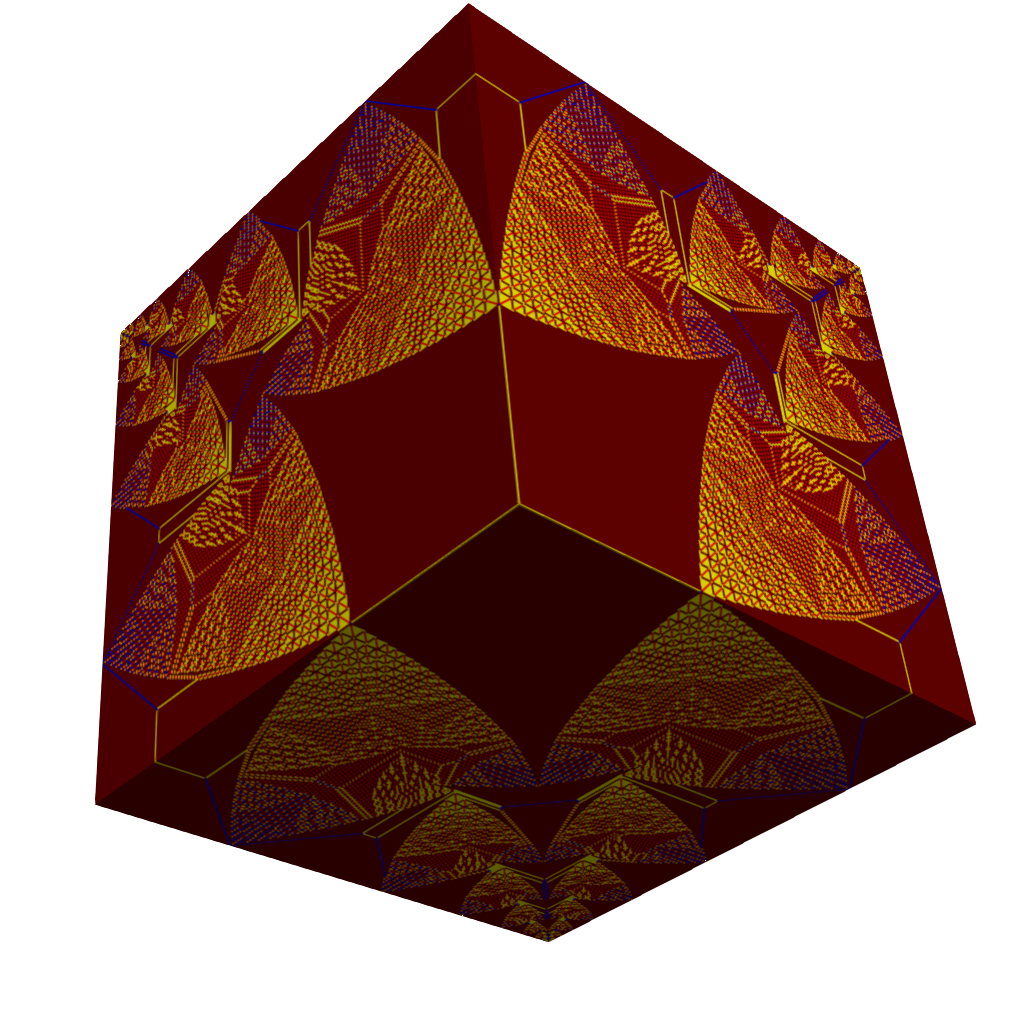
\includegraphics[width = 0.44 \textwidth]{Figures/all7_29.png}}
		\fbox{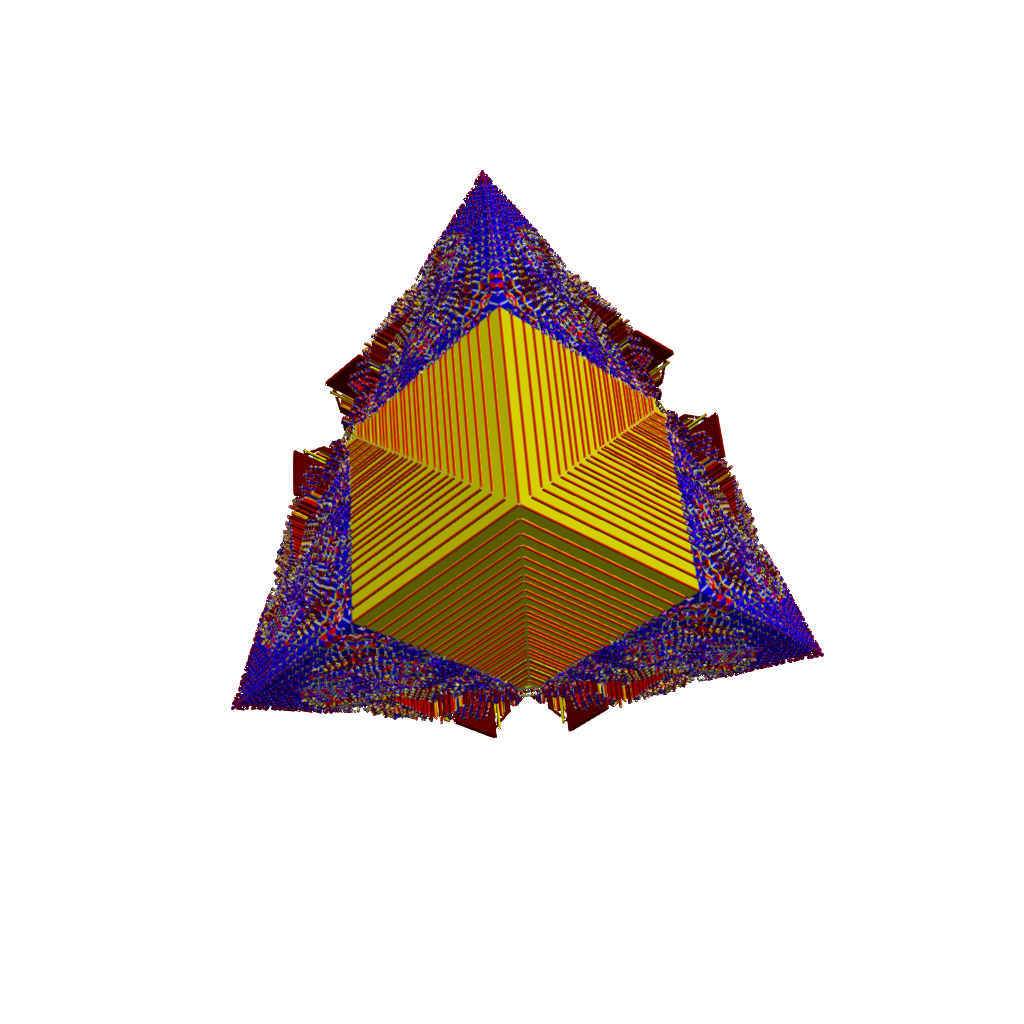
\includegraphics[width = 0.44 \textwidth]{Figures/all7_29_remove.png}}
		\caption{On the left, a corner cube of $s_{\infty}^{(N,3)}$ and on the right the same corner with all cross sections which match 
			$s_{\infty}^{(N,2)}$ removed. The initial condition is $s_0 \equiv 7$ and $N=2^{11}$. Sites with $0,\ldots, 5$ chips are represented by different colors.}
		\label{fig:strong_reduction}
	\end{figure}
	
	
	\begin{problem}
		Extend dimensional reduction on the hypercube to a domain of codimension zero. 
	\end{problem}
	

	
	
	
	\noindent The following is closely related. 
	\begin{problem} \label{prob:c11}
		Show that the odometer for any bounded initial sandpile on the hypercube has bounded second differences. For instance, show 
		for all $t \geq 1$ and $i=1,2$ that 
		\[
		-3 \leq -2 v_t(\mathbf{x}) + v_t(\mathbf{x} + e_i) +v_t(\mathbf{x} - e_i) \leq 2
		\]
		when $d = 2$ and $s_0 \equiv 4$. 
	\end{problem}	
	Numerical evidence indicates the hypercube is a necessary hypothesis in Problem \ref{prob:c11}. In fact, in most other domains, including the discrete circle, the odometer does not appear to have bounded second differences. 
	On the hypercube, our proof of dimensional reduction shows that the odometer has bounded second differences along the central cross sections; however, a method to propagate those bounds to the interior remains out of reach. 

	
	
	
	
	\subsection{Outline of the proof}
	The proof of Theorem \ref{the_theorem} is a careful induction on hypercube dimension, side length, and time. Some parts of the argument can be simplified 
	but we present it in this fashion to suggest a template for proving dimensional reduction with more general initial data. At a high level, 
	we show that if the parallel toppling process for a $d_0$-dimensional sandpile is sufficiently regular, then dimensional reduction is guaranteed 
	in all dimensions $d > d_0$. We prove this regularity when $d_0=1$; the case $d_0 > 1$ remains open. 
	
	
	Our main technical tool is a technique introduced by Babai and Gorodezy to prove discrete quasiconcavity of the single-source sandpile odometer in $\Z^2$ \cite{babai2007sandpile}. By an iteration of their technique, we gain symmetry of the odometer, a derivative comparison result, and a parabolic least action principle. These results, which appear in Section \ref{sec:prelims}, extend beyond the hypercube and so may be of independent interest. 
	
	
	In Section \ref{sec:base_case} we explicitly determine $v_t^{(d,N)}$ when $N=4$ in all dimensions $d \geq 1$ when the initial sandpile is $s_0 \equiv 2 d + d-1$. This is done by 
	mapping the hypercube to a line via a radial decomposition. The explicit form of $v_t$ provides both a base case for our proof and progress towards Problem \ref{prob:true_theorem}.	We also show that when $N=2$ dimensional reduction does not occur at the critical dimension $d_0$. 
	
	The explicit solution when $N=4$ establishes the base case for an odometer regularity result which is then proved in Section \ref{sec:base_regularity}. Finally, in Section \ref{sec:dim_reduction}, we use the established regularity of the odometer in dimension $(d-1)$ to prove dimensional reduction in dimension $d$ 
	
		\subsection*{An efficient algorithm for computing high-dimensional sandpiles}
	In Section \ref{subsec:symmetry} we show that $v_t^{(d,N)}$ can be computed via the parallel toppling procedure restricted to the simplex. In fact, the argument shows that any sandpile with a symmetric initial condition on $\Z^d$, including the single-source sandpile, retains symmetry throughout the parallel toppling process and can be computed in this way. 
	
	For $d$ large, computing sandpiles on the simplex improves space complexity by a factor of $d^d$. Moreover, the reduction in size also leads to a faster algorithm when using parallelization. We wrote a program in Julia \cite{bezanson2017julia, besard2018effective} for computing arbitrary dimensional sandpiles which implements these improvements. The program, which may be freely used and modified, is included in the arXiv post. 
	
	
	\subsection*{Acknowledgements}	
	It is a pleasure to acknowledge Charles K. Smart for encouraging me to work on this problem and for many valuable conversations throughout.
	Additionally, I thank Lionel Levine for helpful discussions and for sharing past, unpublished, joint work with Alexander Holroyd and Karl Mahlburg towards the dimensional reduction conjecture. The anonymous referees provided detailed feedback which led to a much improved exposition.
	
	
	\section{Preliminaries} \label{sec:prelims}
	
	
	\subsection{Notation and conventions}
	When we need to distinguish between vectors and scalars, we reserve $\mathbf{x}$
	for vectors and $x$ for scalars. The $i$-th element of $\mathbf{x}$ is $x_i$
	and $\mathbf{x}_{i} = (x_1, \ldots, x_i)$. We refer to coordinate basis vectors of 
	$\Z^d$ as $e_i$ and the ones vector of length $i$ by
	$\mathbf{1}_{i} = (1, \ldots, 1)$. Equalities, inequalities, addition, and multiplication between vectors and scalars are to be understood pointwise. 
	The notation $|x|$ refers to the absolute value and $|\mathbf{x}| = \sum_{i=1}^d |x_i|$ is the $\ell_1$ norm. 
	
	
	We embed $\mathcal{C}_{N}^{(d)}$ into $\Z^d$ in two different ways depending on whether $N$ is even or odd. If $N = 2 k + 1$,  $\mathcal{C}_N^{(d)} = \{ \mathbf{x} +1 : |x_i| \leq k \}$  otherwise $\mathcal{C}_N^{(d)} = \{ \mathbf{x}-k : 1 \leq x_i \leq 2 k \}$.
	The graph Laplacian on $\mathcal{C}_N^{(d)}$ operates on functions
	$f: \mathcal{C}_N^{(d)} \to \mathbb{R}$ as 
	\begin{equation}
	\Delta^{(d)} f(x) = -2 d f(x) + \sum_{y \sim x} f(y), 
	\end{equation}
	where we pad $f(x) := 0$ for $x \not \in \mathcal{C}_N^{(d)}$ and the 
	sum $y \sim x$ is over the 2d nearest neighbors of $x$, $|y-x| = 1$.  When the hypercube size or dimension is not used, we omit distinguishing sub/superscripts. 
	
	
	\subsection{Babai-Gorodezky technique} 
	In this subsection and the next, let $s_0 \leq 2 (2 d) - 1$ be an arbitrary initial sandpile on $\mathcal{C}$ and $v_t$ its odometer. A straightforward induction argument and the definition of the graph Laplacian yields the following lemma. 
	\begin{lemma}[] \label{pt_ind_lemma}
		For each $x \in \mathcal{C}$ and all $t \geq 0$, 
		\begin{equation}
		v_{t+1}(x) = \max\left\{0,\left\lfloor
        \frac{s_0(x)+\sum_{y\sim x}v_t(y)}{2d}\right\rfloor\right\}.
		\end{equation}
	\end{lemma}
	Babai and Gorodezky used this simple lemma to prove a nontrivial discrete quasiconcavity property of the single-source sandpile in $\Z^d$ \cite{babai2007sandpile}. A more general version of their argument appears below in Lemma \ref{general_difference_comparison}. Roughly, their technique recognizes that if a property of the odometer holds at $t=1$, is consistent across the symmetry axes, and can be verified on the boundaries of the domain, it must hold for all $t \geq 1$.
	
	Lemma \ref{pt_ind_lemma} is used many other times throughout this paper; notably we use it to prove a parabolic least action principle and symmetry of the odometer on the hypercube. 
	
	
	\subsection{Parabolic least action principle} 
	The least action principle \cite{fey2010growth} shows that $v_\infty$ is minimal among all $w: \mathcal{C} \to \mathbb{Z}^+$ which {\it stabilize} $s_0$: $\Delta w + s_0 \leq 2d -1$. We upgrade this to a parabolic least action principle by observing the parallel toppling procedure as a directed sandpile on $\mathcal{G} = \mathbb{Z}^+ \times \mathcal{C}$. The initial sandpile and odometer over time are stacked,
	$s(t,x) := s_0(x)$ and $v(t,x) := v_t(x)$ for all $t \geq 0$ and $x \in \mathcal{C}$.  The graph Laplacian operates on functions $f:\mathcal{G} \to \mathbb{R}$ as
	\begin{equation}
	\Delta^{\mathcal{G}} f(t,x) = -2 d f(t,x) + \sum_{y \sim x} f(t-1,y),
	\end{equation}
	for $t \geq 1$ and $x \in \mathcal{C}$, where the sum $y \sim x$ is over the nearest neighbors of $x$ in $\mathcal{C}$.

	
	
	
	\begin{lemma}[Parabolic least action principle] \label{parabolic_comparison}
		\begin{equation} \label{eq:parabolic_leastaction}
		v(t,x) = \min\{ u: \mathcal{G} \to \mathbb{Z}^+: \Delta^{\mathcal{G}} u(t,x) + s(t,x) \leq 2d-1 \mbox{ for all $x \in \mathcal{C}$ and $t \geq 1$} \}
		\end{equation}
		%If $\Delta^{\mathcal{G}} w + s \leq 2d-1$, then $w(t, \cdot) \geq v_t(\cdot)$ for all $t \geq 1$.
	\end{lemma}
	\begin{proof}
Route: Step 1 shows that $v$ belongs to the class in \eqref{eq:parabolic_leastaction}. Step 2 shows that every member of the class lies above $v$.

\emph{Step 1.} We show that $v$ belongs to the class. Put $K:=2d$ and $a_t(x):=s_0(x)+\sum_{y\sim x}v_t(y)$. The standing assumption is $s_0\leq 2K-1$, so Lemma \ref{pt_ind_lemma} gives $v_{t+1}(x)=\max\{0,\lfloor a_t(x)/K\rfloor\}$. For every integer $a$ we have $\lfloor a/K\rfloor>a/K-1$, so $K\lfloor a/K\rfloor\geq a-(K-1)$. Hence $K v_{t+1}(x)\geq a_t(x)-(K-1)$ for all $t\geq0$ and $x\in\mathcal C_N^{(d)}$. Rearranging gives
\begin{equation*}
-K\,v_{t+1}(x)+\sum_{y\sim x}v_t(y)+s_0(x)\leq K-1\,,
\end{equation*}
which is the constraint at time $t+1$. The values of $v$ are nonnegative integers, so $v$ belongs to the class.

\emph{Step 2.} Let $u$ be any member of the class, and extend $u$ and $v$ by zero outside $\mathcal C_N^{(d)}$. This does not change the neighbour sums in the constraint at points of $\mathcal C_N^{(d)}$. We show by induction on $t$ that $v_t\leq u_t$. At $t=0$ this holds since $v_0=0$ and $u_0\geq0$. Assume $v_t\leq u_t$. Both functions vanish outside $\mathcal C_N^{(d)}$, so the inequality holds on all of $\mathbb Z^d$. Fix $y\in\mathcal C_N^{(d)}$ and put
\begin{equation*}
b:=s_0(y)+\sum_{y'\sim y}u_t(y')\,,\qquad a:=s_0(y)+\sum_{y'\sim y}v_t(y')\,.
\end{equation*}
The constraint for $u$ at time $t+1$ says $b\leq Ku_{t+1}(y)+K-1$, that is, $b<K\big(u_{t+1}(y)+1\big)$. Since $a\leq b$, we get $a<K\big(u_{t+1}(y)+1\big)$, and therefore $\lfloor a/K\rfloor\leq u_{t+1}(y)$. Together with $u_{t+1}(y)\geq0$, this gives $v_{t+1}(y)=\max\{0,\lfloor a/K\rfloor\}\leq u_{t+1}(y)$. This completes the induction.

By Steps 1 and 2, $v$ belongs to the class and lies below each of its members. So $v$ is the pointwise minimum of the class, which is \eqref{eq:parabolic_leastaction}.
    \end{proof}
	\noindent  
	Our usage of the parabolic least action principle in the main argument is minimal
	and can be avoided. And, in some sense, it is a restatement of Lemma \ref{pt_ind_lemma}. We included it as it may be of independent interest. 
	
	\subsection{Symmetry and fundamental domains} \label{subsec:symmetry}
	In this section we observe that sandpile dynamics on $\mathcal{C}_N^{(d)}$ preserve the symmetry structure of the $d$-dimensional hypercube.
	This is then used to reduce to the sandpile on a {\it fundamental domain} of the hypercube with reflecting boundary conditions.  The main contribution 
	of this subsection is a coordinate-wise description of this domain along with an explicit formula for the reflecting graph Laplacian. 
	
	We briefly provide a presentation of the group of automorphisms of the hypercube
	and its action on $\Z^d$; for more details see, for example, \cite{godsil2013algebraic}. 
	Let $\operatorname{Aut}_{\mathcal{C}_d}$ be the group of $(d \times d)$ matrices 
	with exactly one $\pm 1$ in each row and in each column and $0$s elsewhere. 
	Let $\sigma \in \operatorname{Aut}_{\mathcal{C}_d}$ act on $x \in \Z^d$ by matrix-vector multiplication
	followed by a translation and let it act on $f:\Z^d \to \mathbb{R}$ by $\sigma f(x) := f(\sigma x)$. 
	The translation is chosen to preserve $\mathcal{C}_{N}^{(d)}$ when $N$ is even or odd in our choice of coordinates. 

	% when it is even you can add 1/2 to all coordinates of Z^d and then 
	
	Each $\sigma$ is an isometry and hence preserves nearest neighbors and $\mathcal{C}^{(d)}_N$. 
	That is, if $y \not \in \mathcal{C}^{(d)}_{N}$, then $\sigma y \not \in \mathcal{C}^{(d)}_{N}$.
	And, if $|y-x| = 1$, then $|\sigma y - \sigma x| = 1$, so 
	\begin{equation} \label{eq:isometry}
	\sum_{y' \sim \sigma x} f(y') = \sum_{y \sim x} f(\sigma y).
	\end{equation}
	
	
	We say $\Omega \subseteq \mathcal{C}_{N}^{(d)}$ is a fundamental domain if there exists a set $\{\sigma_1, \sigma_2, \ldots \}  \subset  \operatorname{Aut}_{\mathcal{C}_d}$ so that $\bigcup_j \sigma_j \Omega = \mathcal{C}_{N}^{(d)}$. For example, a fundamental domain of an interval is half of it, 
	while a fundamental domain of a square is a right triangle with one side along a central cross section of the square. The fundamental domains which we consider have coordinate consistency across dimensions.  Let $M = \lceil N/2 \rceil$ and 
	\begin{equation}
	\mathcal{S}^{(d)}_M := \{ (x_1, \ldots, x_d): M \geq x_1 \geq \cdots \geq x_d \geq 1 \}.
	\end{equation}
	Observe that  $\{ \mathbf{x}_{d-1} : (\mathbf{x}_{d-1}, 1) \in \mathcal{S}^{(d)}_M\} = \mathcal{S}^{(d-1)}_M$;
	this is the first step towards proving dimensional reduction on the hypercube. 
	
	Let $s_0:\mathcal{C}_N^{(d)}\to\mathbb Z$ be invariant under the cube
    symmetries on its cube domain. Every site $y$ in the cube has a unique
    orbit representative $r_N(y)\in\mathcal{S}^{(d)}_M$; the symmetry taking
    $y$ to that representative need not be unique. For
    $u:\mathcal{S}^{(d)}_M\to\mathbb Z$ define its lifted values by
    \[
    \widetilde u(y)=\begin{cases}u(r_N(y)),&y\in\mathcal{C}_N^{(d)},\\
    0,&y\notin\mathcal{C}_N^{(d)}.\end{cases}
    \]
    Write $R u(x)=\sum_{i=1}^d(\widetilde u(x+e_i)+\widetilde u(x-e_i))$.
    The sum retains all $2d$ directed occurrences, including repeated orbit
    representatives and zero contributions from exterior neighbors. Define
    the symmetrized odometer independently by $v_0^{\mathcal S}\equiv0$ and
    \[
    v_{t+1}^{\mathcal S}(x)=v_t^{\mathcal S}(x)+
    1\{s_0(x)+R v_t^{\mathcal S}(x)-2d v_t^{\mathcal S}(x)\geq2d\}.
    \]
    This uses the physical cube embedding for each parity of $N$: reflection
    sends $0$ to $1$ for even $N$ and $0$ to $2$ for odd $N$.


	
	%The symmetric graph Laplacian is then defined as,
	%\begin{equation}
	%\Delta^{\mathcal{S}} v_t^{\mathcal{S}}(x) = -2d v_t^{\mathcal{S}}(x) + \sum_{y \overset{\mathcal{S}}{\sim}  x} v_t^{\mathcal{S}}(y).
	%\end{equation}
		
	
	
	\begin{lemma}[Symmetry]\label{symmetry_lemma}
		For each $t \geq 0$ and each $ \sigma \in \operatorname{Aut}_{\mathcal{C}_d}$, $ \sigma v_t = v_t$. Hence, $v_t = v_t^{\mathcal{S}}$ on $\mathcal{S}^{(d)}_M$.
	\end{lemma}
	
	\begin{proof}
Route: Step 1 proves the invariance $\sigma v_t=v_t$ by induction on $t$. Step 2 shows, again by induction on $t$, that the physical odometer on $\mathcal S$ follows the recursion defining $v^{\mathcal S}$.

\emph{Step 1.} We show that $\sigma v_t=v_t$ for every $\sigma\in\operatorname{Aut}_{\mathcal C_d}$ and every $t\geq0$. The zero odometer is invariant. Assume $v_t(\sigma x)=v_t(x)$ for all $x$ and all $\sigma$. Each $\sigma$ maps $\mathcal C_N^{(d)}$ onto itself, and it carries the $2d$ directed neighbours of $x$ bijectively onto those of $\sigma x$, so $\sum_{y'\sim\sigma x}v_t(y')=\sum_{y\sim x}v_t(\sigma y)$. The initial pile is invariant, $s_0(\sigma x)=s_0(x)$. Hence the height at time $t$ satisfies
\begin{equation*}
s_t(\sigma x)=s_0(\sigma x)-2d\,v_t(\sigma x)+\sum_{y\sim x}v_t(\sigma y)=s_t(x)\,,
\end{equation*}
by the induction hypothesis. The odometer rule then gives $v_{t+1}(\sigma x)=v_{t+1}(x)$ for $x\in\mathcal C_N^{(d)}$. Outside the cube both values are zero.

\emph{Step 2.} We show that $v_t(x)=v_t^{\mathcal S}(x)$ for every $x\in\mathcal S$ and every $t\geq0$. Both sides vanish at $t=0$. Assume the identity at time $t$. For $y\in\mathcal C_N^{(d)}$ let $r_N(y)\in\mathcal S$ be its orbit representative. By Step 1, $v_t(y)=v_t(r_N(y))=v_t^{\mathcal S}(r_N(y))$, and $v_t(y)=0$ outside the cube, so $v_t$ is the lift of $v_t^{\mathcal S}$ defined above. For $x\in\mathcal S$ the $2d$ neighbours of $x$ therefore contribute $\sum_{y\sim x}v_t(y)=R\,v_t^{\mathcal S}(x)$, and the exterior neighbours contribute zero. Thus the physical update at $x$ reads
\begin{equation*}
v_{t+1}(x)=v_t(x)+\mathbf 1\{s_0(x)+R\,v_t^{\mathcal S}(x)-2d\,v_t^{\mathcal S}(x)\geq 2d\}=v_{t+1}^{\mathcal S}(x)\,,
\end{equation*}
which is exactly the recursion defining $v^{\mathcal S}$. This completes the induction.

Hence $v_t=v_t^{\mathcal S}$ on $\mathcal S$ for every $t\geq0$.
    \end{proof}
	\noindent Note that the proof indicates that Lemma \ref{symmetry_lemma} can be extended in a natural way to 
	other graphs and domains which are preserved under the automorphism group of the graph. 
	
	
	Henceforth, we consider $v_t^{\mathcal{S}}$ in $\mathcal{S}_M^{(d)}$ and drop all $\mathcal{S}$ superscripts. To reduce the number of cases with similar 
	arguments, we only consider $N = 2 M$. Indeed, when $N$ is odd, the proofs
	are identical except for slight changes to the boundary arguments. Also, we will use $\mathcal{S}_M^{(d)}$ to refer exclusively to the sorted fundamental domain of $\mathcal{C}_{2M}^{(d)}$. The expressions $v_t^{(d,M)}$  and $s_t^{(d,M)}$ will refer to the parallel toppling odometers and sandpiles on $\mathcal{S}_M^{(d)}$. 
	
	
	\subsection{Derivative comparison}
	In this section we provide a general parabolic comparison result for first order differences of $v_t$ on $\mathcal{S}_M$
	when the initial sandpile, $s_0$, is constant. For $w \in \Z^d$, let $D_{w}$ denote a first order difference operator of the form $D_{w} v_t(\cdot) = v_t(\cdot) - v_t(\cdot+w)$. Pad $v_t$ by $v_t(x) := 0$ for all $x \not \in \mathcal{C}_N$.  
	Denote the interior with respect to $w$ as 
	\begin{equation}
	\mbox{Int}_w(\mathcal{S}_M) = \{ x \in \mathcal{S}_M : y' \in \mathcal{S}_M \mbox{ for all $|y'-(x+w)| = 1$} \}
	\end{equation}
	and the boundary as 
	\begin{equation}
	\partial_w \mathcal{S}_M = \mathcal{S}_M \backslash \mbox{Int}_w(\mathcal{S}_M).  
	\end{equation}

	
	Observe that every symmetrized $y \sim x \in \mathcal{S}_M$ is of the form $y = (x \pm e_i) \mp d_i$,  where $d_i$ is either a reflection, $d_i = e_i$ or a 
	rotation $d_i = e_i -e_j$. We will show that if one can control $D_{w} v_t$ over the reflecting, rotating, and dissipating boundaries of $\mathcal{S}_M$, then that control persists over time. The dissipating boundary on $\mathcal{S}_M$ is
	\begin{equation} \label{eq:dissipative_boundary}
	\mathcal{B}^{(disp)}_w \mathcal{S}_M = \{ x \in \mathcal{S}_M : (x + w)_{i} \geq M  \mbox{ for some $1 \leq i \leq d$} \}
	\end{equation}
	while the reflecting and rotating boundaries are  
	\begin{equation} \label{eq:reflecting_boundary}
	\mathcal{B}^{(ref)}_w \mathcal{S}_M = \{ x \in \mathcal{S}_M : (x+w)_{i} \leq 1 \mbox{ for some $1 \leq i \leq d$} \}
	\end{equation}
	and
	\begin{equation} \label{eq:rotating_boundary}
	\mathcal{B}^{(rot)}_w \mathcal{S}_M = \{ x \in \mathcal{S}_M : (x+w)_i \leq (x + w)_j \mbox{ for some $1 \leq i < j \leq d$} \}.
	\end{equation}
	For notational convenience write
	\begin{equation} \label{eq:all_boundaries}
	\mathcal{B}_w = \{\mathcal{B}^{(disp)}_{w}  \cup \mathcal{B}^{(ref)}_{w} \cup \mathcal{B}^{(rot)}_{w} \}
	\end{equation}
	and  $\mathcal{B}_{w_1, \ldots, w_n} = \cup_{i=1}^n \mathcal{B}_{w_i}$
	for points $w_i \in \Z^d$. 
		Note that in next lemma, we employ our convention to sometimes omit distinguishing sub/superscripts. 
	
	\begin{lemma} \label{general_difference_comparison}
		Let  $\mathbf{w} := \{w_1, \ldots, w_n\}$ be a set of points in $\Z^d$ each equipped with a function $g_j: \mathcal{S} \to \Z$ which is superharmonic in the interior of $\mathcal{S}$. If	
		\begin{equation}
		\label{eq:initial_cond} \sup_{j} \left( D_{w_j} v_{t_0}(x) - g_j(x) \right)  \leq 0 \mbox{\qquad for all $x \in \mathcal{S}$}
		\end{equation}
		and for all $t \geq t_0$ and $x \in \{\mathcal{B}_0 \cup \mathcal{B}_{\mathbf{w}}\} \mathcal{S}$,
		\begin{equation} \label{eq:boundaries_ref}
		\begin{aligned}
		\sup_j &\left(\sum_{y\sim x}v_t(y)-\sum_{y'\sim(x+w_j)}v_t(y')
        -2d g_j(x)\right)\leq0
        \quad\mbox{and $x+w_j\in\mathcal C_N^{(d)}$ for every $j$}\\
		&\mbox{  \qquad or } \\
		\sup_{j}  &( D_{w_j} v_{t+1}(x) - g_j(x) ) \leq 0
		 \end{aligned}
		\end{equation}
		then
		\begin{equation} \label{eq:derivative_comparison}
		\sup_{j} \left( D_{w_j} v_{t+1}(x) - g_j(x) \right) \leq 0
		\end{equation}
		for all $t \geq t_0$ and $x \in \mathcal{S}$. 
		
	\end{lemma}
	
	\begin{proof}
	We induct on $t\geq t_0$. The case $t=t_0$ is \eqref{eq:initial_cond}. Fix $t\geq t_0$ and assume $D_{w_j}v_t\leq g_j$ on $\mathcal S$ for every $j$. We prove the same inequality at time $t+1$ in three steps. Step 1 is a one-step estimate for a pair of sites. Steps 2 and 3 treat the interior and boundary points of $\mathcal S$, and each applies Step 1.
	
	\emph{Step 1.} We show that if $x,y\in\mathcal C_N^{(d)}$ and $a\in\Z$ satisfy
	\begin{equation*}
	v_t(x)-v_t(y)\leq a
	\quad\mbox{and}\quad
	\sum_{x'\sim x}v_t(x')-\sum_{y'\sim y}v_t(y')\leq 2d\,a\,,
	\end{equation*}
	then $v_{t+1}(x)-v_{t+1}(y)\leq a$.
	
	For $z\in\mathcal C_N^{(d)}$, the height of $z$ at time $t$ is
	\begin{equation*}
	s_t(z)=s_0(z)-2d\,v_t(z)+\sum_{y\sim z}v_t(y)\,.
	\end{equation*}
	The odometer rule $v_{t+1}(z)=v_t(z)+\mathbf{1}\{s_t(z)\geq 2d\}$ says that $z$ topples at step $t+1$ exactly when $s_t(z)\geq 2d$. In particular, $v_{t+1}(z)-v_t(z)\in\{0,1\}$.
	
	Suppose first that $v_t(x)-v_t(y)<a$. Both sides are integers, so $v_t(x)-v_t(y)\leq a-1$. Since $v_{t+1}(x)-v_t(x)\leq 1$ and $v_{t+1}(y)-v_t(y)\geq 0$, we get $v_{t+1}(x)-v_{t+1}(y)\leq v_t(x)-v_t(y)+1\leq a$.
	
	Suppose next that $v_t(x)-v_t(y)=a$. The initial sandpile $s_0$ is constant, so $s_0(x)=s_0(y)$. The heights therefore satisfy
	\begin{equation*}
	s_t(x)-s_t(y)=\Big(\sum_{x'\sim x}v_t(x')-\sum_{y'\sim y}v_t(y')\Big)-2d\,\big(v_t(x)-v_t(y)\big)\leq 2d\,a-2d\,a=0\,.
	\end{equation*}
	Hence $s_t(x)\leq s_t(y)$, so if $x$ topples at step $t+1$, then $s_t(y)\geq s_t(x)\geq 2d$ and $y$ topples at step $t+1$ too. Thus $v_{t+1}(x)-v_t(x)\leq v_{t+1}(y)-v_t(y)$, and
	\begin{equation*}
	v_{t+1}(x)-v_{t+1}(y)=\big(v_t(x)-v_t(y)\big)+\big(v_{t+1}(x)-v_t(x)\big)-\big(v_{t+1}(y)-v_t(y)\big)\leq a\,.
	\end{equation*}
	This proves Step 1.
	
	\emph{Step 2.} We show the inequality at every $x\in\mathcal S$ with $x\notin\mathcal B_0\cup\mathcal B_{\mathbf w}$. Fix such an $x$ and an index $j$. Since $x\notin\mathcal B_0$, we have $1<x_i<M$ for all $i$ and $x_j<x_i$ for $i<j$, which gives $x\pm e_i\in\mathcal S$ for every $i$. Since $x\notin\mathcal B_{\mathbf w}$, the same strict inequalities hold at $x+w_j$, so $x+w_j\in\mathcal S$. Summing the induction hypothesis $D_{w_j}v_t(y)\leq g_j(y)$ over the neighbours $y$ of $x$ gives
	\begin{equation*}
	\sum_{y\sim x}v_t(y)-\sum_{y'\sim x+w_j}v_t(y')=\sum_{y\sim x}\big(v_t(y)-v_t(y+w_j)\big)\leq\sum_{y\sim x}g_j(y)\leq 2d\,g_j(x)\,.
	\end{equation*}
	The equality substitutes $y'=y+w_j$, which runs over the neighbours of $x+w_j$ as $y$ runs over the neighbours of $x$. The last inequality is the superharmonicity of $g_j$ at $x$. Now Step 1 applies with $y=x+w_j$ and $a=g_j(x)$. Its first hypothesis is the induction hypothesis at $x$, and its second is the display above. Hence $D_{w_j}v_{t+1}(x)\leq g_j(x)$.
	
	\emph{Step 3.} We show the inequality at every $x\in\mathcal S\cap(\mathcal B_0\cup\mathcal B_{\mathbf w})$. The hypothesis \eqref{eq:boundaries_ref} at time $t$ gives one of its two alternatives. If the second alternative holds, the inequality at time $t+1$ is part of the hypothesis. If the first holds, then $x+w_j\in\mathcal C_N^{(d)}$ for every $j$, and the neighbour inequality holds with $2d\,g_j(x)$ on the right. Step 1 with $y=x+w_j$ and $a=g_j(x)$, together with the induction hypothesis at $x$, gives $D_{w_j}v_{t+1}(x)\leq g_j(x)$ for every $j$.
	
	Steps 2 and 3 cover all of $\mathcal S$, which completes the induction.
	\end{proof}
	
	\noindent As a corollary, we deduce the following discrete quasiconcavity property of $v_t$ on a hypercube, which was proved in \cite{babai2007sandpile}
	for axis monotonic initial sandpiles on $\Z^2$.  (Note that Aleksanyan and Shahgholian, using a discrete analogue of the method of moving planes, proved axis monotonicity
	of $v_{\infty}$ in \cite{aleksanyan2019discrete}.)
	\begin{corollary}[Axis monotonicity \cite{babai2007sandpile}] \label{axis_monotonicity}
		For all $t\geq1$, $x\in\mathcal S$, every $1\leq i\leq d$, and
        $\mathcal J=\varnothing$ or $\mathcal J=\{j\}$ with $i<j\leq d$,
        \[
        v_t(x)\geq v_t(x+e_i-e_{\mathcal J})
        \quad\mbox{when $x+e_i-e_{\mathcal J}\in\mathcal S$},
        \]
        where $e_{\mathcal J}=\sum_{k\in\mathcal J}e_k$.
        In particular, iteration gives the pure-coordinate monotonicity
        for any sequence of steps away from reflection mirrors.
	\end{corollary}

	\begin{proof}
Route: Step 1 proves the reflection comparison and Step 2 the interchange comparison, each for all $t\geq0$ and all $x\in\mathbb Z^d$, with $v_t$ extended by zero. Step 3 specialises them to the corollary. Throughout this subsection $s_0$ is constant.

\emph{Step 1 (reflection comparison).} We show that $v_t(x+e_i)\leq v_t(x)$ whenever $x_i\geq1$. This holds at $t=0$, so assume it at time $t$ for all $x$. If $x\notin\mathcal C_N^{(d)}$, then $x+e_i\notin\mathcal C_N^{(d)}$, because $x_i\geq1$ and moving up in coordinate $i$ cannot bring an out-of-range coordinate back into range. Both values vanish at time $t+1$. If $x\in\mathcal C_N^{(d)}$ and $x+e_i\notin\mathcal C_N^{(d)}$, then $v_{t+1}(x+e_i)=0\leq v_{t+1}(x)$. Now let both points lie in the cube.

If $v_t(x+e_i)<v_t(x)$, then integrality and $v_{t+1}(z)-v_t(z)\in\{0,1\}$ give $v_{t+1}(x+e_i)\leq v_t(x+e_i)+1\leq v_t(x)\leq v_{t+1}(x)$.

If $v_t(x+e_i)=v_t(x)$, we compare heights. For each $k$, the two neighbours $x+e_i\pm e_k$ of $x+e_i$ are paired with $x+e_k$ and $x-e_k$. The induction hypothesis at $x+e_k$ gives $v_t(x+e_i+e_k)\leq v_t(x+e_k)$, and the hypothesis at $x-e_k$ gives $v_t(x+e_i-e_k)\leq v_t(x-e_k)$ when $x-e_k$ has $i$-th coordinate at least $1$. The only exception is $k=i$ with $x_i=1$. In that case $v_t(x-e_i)=v_t(x)$, by Lemma \ref{symmetry_lemma} applied to the reflection $y_i\mapsto 1-y_i$, which exchanges $x$ and $x-e_i$. So in all cases $v_t(x+e_i+e_k)+v_t(x+e_i-e_k)\leq v_t(x+e_k)+v_t(x-e_k)$. Summing over $k$ gives $\sum_{y\sim x+e_i}v_t(y)\leq\sum_{y\sim x}v_t(y)$. With $s_0$ constant and $v_t(x+e_i)=v_t(x)$, the heights satisfy $s_t(x+e_i)\leq s_t(x)$. So if $x+e_i$ topples at step $t+1$, then $x$ topples too, and $v_{t+1}(x+e_i)\leq v_{t+1}(x)$.

\emph{Step 2 (interchange comparison).} We show that $v_t(x+e_i-e_j)\leq v_t(x)$ whenever $i\neq j$ and $x_j\leq x_i$. This holds at $t=0$, so assume it at time $t$ for all such $x$. Write $y:=x+e_i-e_j$. If $y\notin\mathcal C_N^{(d)}$, then $v_{t+1}(y)=0\leq v_{t+1}(x)$. If $y\in\mathcal C_N^{(d)}$, then $x\in\mathcal C_N^{(d)}$ as well, because $y_j<x_j\leq x_i<y_i$, so both coordinates of $x$ are in range. Now let both points lie in the cube.

If $v_t(y)<v_t(x)$, the same integrality argument gives $v_{t+1}(y)\leq v_{t+1}(x)$.

If $v_t(y)=v_t(x)$, we compare heights. For each $k$, the neighbours $y\pm e_k$ of $y$ are paired with $x+e_k$ and $x-e_k$. For $y+e_k$ and $x+e_k$ with $k\neq j$, the hypothesis at $x+e_k$ applies, because $(x+e_k)_j=x_j\leq x_i\leq(x+e_k)_i$. For $k=j$, the pair is $x+e_i$ and $x+e_j$. If $x_j<x_i$, the hypothesis at $x+e_j$ gives $v_t(x+e_i)\leq v_t(x+e_j)$. If $x_j=x_i$, the transposition of coordinates $i$ and $j$ fixes $x$ and carries $x+e_i$ to $x+e_j$, so Lemma \ref{symmetry_lemma} gives equality. For $y-e_k$ and $x-e_k$ with $k\neq i$, the hypothesis at $x-e_k$ applies, because $(x-e_k)_j\leq x_j\leq x_i=(x-e_k)_i$. For $k=i$, the pair is $x-e_j$ and $x-e_i$. If $x_j<x_i$, the hypothesis at $x-e_i$ gives $v_t(x-e_j)\leq v_t(x-e_i)$. If $x_j=x_i$, the transposition gives equality as before. Summing over $k$ shows $\sum_{y'\sim y}v_t(y')\leq\sum_{y'\sim x}v_t(y')$. Hence $s_t(y)\leq s_t(x)$, and the toppling argument of Step 1 gives $v_{t+1}(y)\leq v_{t+1}(x)$.

\emph{Step 3.} Let $x\in\mathcal S$, $1\leq i\leq d$, and $\mathcal J=\varnothing$ or $\mathcal J=\{j\}$ with $i<j$. If $\mathcal J=\varnothing$, then $x_i\geq1$ and Step 1 gives the claim. If $\mathcal J=\{j\}$, then $x_i\geq x_j$ because $x\in\mathcal S$, and Step 2 gives the claim. This proves the corollary.
    \end{proof}
		\begin{corollary}[Derivative bound] \label{cor:derivative_bound}
		Suppose $v_{\infty}(M, \mathbf{1}_{d-1}) \leq k M$ for integer $k \geq 1$. 
		Then, for all $1 \leq j \leq d$ and $t \geq 0$
		\begin{equation} \label{eq:cor:derivative_bound}
		v_t(x) - v_t(x+e_j) \leq k x_j.
		\end{equation}

	\end{corollary}
	
	\begin{proof}
The proof has two parts. Step 1 bounds $v_t$ on the top face $\{x_j=M\}$ by the corner hypothesis. Steps 2 to 5 prove the inequality by induction on $t$ for all $x \in \mathbb{Z}^d$ with $x_j \geq 1$, not only for $x \in \mathcal{S}$, because the induction step uses neighbours that can leave $\mathcal{S}$ or the cube.

\emph{Step 1.} We show that $v_t(x) \leq kM$ for all $t \geq 0$ and every $x \in \mathcal{C}_N^{(d)}$ with $x_j = M$. Put $\mathbf{c} = (M, \mathbf{1}_{d-1})$. The odometer is nondecreasing in time, so $v_t(\mathbf{c}) \leq v_\infty(\mathbf{c}) \leq kM$. Folding each coordinate $c \leq 0$ to $1-c$ and then sorting the coordinates in decreasing order gives a symmetry $\sigma$ with $y := \sigma x \in \mathcal{S}$, and Lemma \ref{symmetry_lemma} gives $v_t(x) = v_t(y)$. The folded value of $x_j$ is $M$, so $y_1 = M$.

Now walk from $y$ to $\mathbf{c}$ inside $\mathcal{S}$. Let $z \in \mathcal{S}$ with $z \neq \mathbf{c}$, and let $l$ be the largest index with $z_l > 1$. Then $l \geq 2$, and $z - e_l \in \mathcal{S}$, because $z_{l-1} \geq z_l > z_l - 1 \geq 1 = z_{l+1}$ (the last comparison is void when $l = d$). Corollary \ref{axis_monotonicity} with $\mathcal{J} = \varnothing$ gives $v_t(z - e_l) \geq v_t(z)$ for $t \geq 1$, and both sides vanish at $t = 0$. So $v_t$ does not decrease along the walk, which ends at $\mathbf{c}$. Hence $v_t(x) = v_t(y) \leq v_t(\mathbf{c}) \leq kM$.

\emph{Step 2.} For $t \geq 0$ let $P(t)$ be the statement that $v_t(x) - v_t(x+e_j) \leq k\,x_j$ for every $j \in \{1, \ldots, d\}$ and every $x \in \mathbb{Z}^d$ with $x_j \geq 1$, where $v_t$ is extended by zero outside $\mathcal{C}_N^{(d)}$. The statement $P(0)$ holds because $v_0 \equiv 0$ and $k\,x_j \geq 0$. Assume $P(t)$, fix $j$ and $x$ with $x_j \geq 1$, and put $D := v_t(x) - v_t(x+e_j)$. We show that $v_{t+1}(x) - v_{t+1}(x+e_j) \leq k\,x_j$.

\emph{Step 3.} This step treats the cases in which $x$ or $x+e_j$ lies outside the cube. If $x \notin \mathcal{C}_N^{(d)}$, then $v_{t+1}(x) = 0$, and the difference is $-v_{t+1}(x+e_j) \leq 0 \leq k\,x_j$. If $x \in \mathcal{C}_N^{(d)}$ but $x+e_j \notin \mathcal{C}_N^{(d)}$, then $x_j = M$, so $v_{t+1}(x+e_j) = 0$ and Step 1 gives $v_{t+1}(x) \leq kM = k\,x_j$.

\emph{Step 4.} Assume from now on that $x$ and $x+e_j$ both lie in the cube. The height of $z$ at time $t$ is $s_t(z) = s_0(z) - 2d\,v_t(z) + \sum_{y \sim z} v_t(y)$, and the odometer rule $v_{t+1}(z) = v_t(z) + \mathbf{1}\{s_t(z) \geq 2d\}$ gives $v_{t+1}(z) - v_t(z) \in \{0, 1\}$. The number $D$ is an integer with $D \leq k\,x_j$ by $P(t)$. If $D < k\,x_j$, then $D \leq k\,x_j - 1$, and therefore $v_{t+1}(x) - v_{t+1}(x+e_j) \leq D + 1 \leq k\,x_j$.

\emph{Step 5.} Assume finally that $D = k\,x_j$. For $i \in \{1, \ldots, d\}$ put
\begin{equation*}
B_i := \big(v_t(x+e_i) - v_t(x+e_i+e_j)\big) + \big(v_t(x-e_i) - v_t(x-e_i+e_j)\big)\,.
\end{equation*}
We claim that $B_i \leq 2k\,x_j$. If $i \neq j$, then $P(t)$ at $x+e_i$ and at $x-e_i$, whose $j$-th coordinates are both $x_j \geq 1$, bounds each bracket by $k\,x_j$. If $i = j$ and $x_j \geq 2$, then $P(t)$ at $x+e_j$ and at $x-e_j$, whose $j$-th coordinates are $x_j+1$ and $x_j-1$, bounds the brackets by $k(x_j+1)$ and $k(x_j-1)$. If $i = j$ and $x_j = 1$, the reflection $y_j \mapsto 1-y_j$ fixes the cube and exchanges $x-e_j$ and $x$, so $v_t(x-e_j) = v_t(x)$ by Lemma \ref{symmetry_lemma}. The second bracket then vanishes, and $P(t)$ at $x+e_j$ bounds the first by $k(x_j+1) = 2k\,x_j$.

The neighbours of $x$ are $x \pm e_i$, and the neighbours of $x+e_j$ are $x+e_j \pm e_i$. Hence
\begin{equation*}
\sum_{y \sim x} v_t(y) - \sum_{y \sim x+e_j} v_t(y) = \sum_{i=1}^d B_i \leq 2d\,k\,x_j\,.
\end{equation*}
Since $s_0$ is constant, the heights satisfy
\begin{equation*}
s_t(x) - s_t(x+e_j) = \Big(\sum_{y \sim x} v_t(y) - \sum_{y \sim x+e_j} v_t(y)\Big) - 2d\,D \leq 2d\,k\,x_j - 2d\,k\,x_j = 0\,.
\end{equation*}
So $s_t(x) \leq s_t(x+e_j)$. If $x$ topples at step $t+1$, that is $s_t(x) \geq 2d$, then $s_t(x+e_j) \geq 2d$ and $x+e_j$ topples at step $t+1$ too. Hence $\mathbf{1}\{s_t(x) \geq 2d\} \leq \mathbf{1}\{s_t(x+e_j) \geq 2d\}$, and
\begin{equation*}
v_{t+1}(x) - v_{t+1}(x+e_j) = D + \mathbf{1}\{s_t(x) \geq 2d\} - \mathbf{1}\{s_t(x+e_j) \geq 2d\} \leq D = k\,x_j\,.
\end{equation*}
This proves $P(t+1)$. Hence $P(t)$ holds for every $t$, which gives \eqref{eq:cor:derivative_bound} for all $x \in \mathbb{Z}^d$ with $x_j \geq 1$, in particular for all $x \in \mathcal{S}$.
    \end{proof}
	
	
	\subsection{Weak topple control}	
	We provide a difference-in-time analogue of Lemma \ref{general_difference_comparison}

	\begin{lemma} \label{topple_limit}
	For all $t \geq t_0$ and $j \geq 0$, 
	\[
	\max_{z \in \mathcal{S}} \left( v_{t+j}(z) - v_t(z) \right) \leq \max_{z \in \mathcal{S}} \left( v_{t_0+j}(z) - v_{t_0}(z) \right)
	\]
	%Moreover, $v_{t+j}(x) - v_t(x) = j$ if and only if 
	%$v_{t+j-1}(y) = v_{t-1}(y) + j$ for some neighbor $y \sim x$. 
	\end{lemma}

	
	\begin{proof}
Route: Step 1 bounds the increment over the whole cube by the right-hand maximum $C$. Step 2 shows by induction on $n$ that this bound persists from the pair of times $(t_0+n+j,\,t_0+n)$ to the next pair. Step 3 takes $n=t-t_0$.

\emph{Step 1.} Let $C$ be the right-hand maximum. It is attained on the nonempty finite set $\mathcal S$, and $C\geq0$, because the odometer is nondecreasing in time. We show that $v_{t_0+j}(y)-v_{t_0}(y)\leq C$ for every $y\in\mathbb Z^d$. If $y\notin\mathcal C_N^{(d)}$, the left side is zero. If $y\in\mathcal C_N^{(d)}$, Lemma \ref{symmetry_lemma} shows that the left side equals its value at the representative $z\in\mathcal S$ of $y$, which is at most $C$ by the definition of $C$.

\emph{Step 2.} We show by induction on $n\geq0$ that $v_{t_0+n+j}(y)-v_{t_0+n}(y)\leq C$ for every $y\in\mathbb Z^d$. The case $n=0$ is Step 1. Assume the claim for $n$, and write $a:=t_0+n+j$ and $b:=t_0+n$, so that $v_a(z)-v_b(z)\leq C$ for all $z\in\mathbb Z^d$. We bound $v_{a+1}(y)-v_{b+1}(y)$. If $y\notin\mathcal C_N^{(d)}$, this difference is zero. Let $y\in\mathcal C_N^{(d)}$ and put $D:=v_a(y)-v_b(y)\leq C$.

If $D<C$, then $D\leq C-1$, because both sides are integers. Since $v_{a+1}(y)-v_a(y)\leq1$ and $v_{b+1}(y)-v_b(y)\geq0$, we get $v_{a+1}(y)-v_{b+1}(y)\leq D+1\leq C$.

If $D=C$, we compare heights. Each of the $2d$ neighbours $z\sim y$ satisfies $v_a(z)-v_b(z)\leq C$, so $\sum_{z\sim y}v_a(z)-\sum_{z\sim y}v_b(z)\leq 2d\,C$. The initial pile $s_0(y)$ is the same at both times, so
\begin{equation*}
s_a(y)-s_b(y)=\Big(\sum_{z\sim y}v_a(z)-\sum_{z\sim y}v_b(z)\Big)-2d\,D\leq 2d\,C-2d\,C=0\,.
\end{equation*}
Hence $s_a(y)\leq s_b(y)$, so $\mathbf 1\{s_a(y)\geq 2d\}\leq\mathbf 1\{s_b(y)\geq 2d\}$. The odometer rule gives
\begin{equation*}
v_{a+1}(y)-v_{b+1}(y)=D+\mathbf 1\{s_a(y)\geq 2d\}-\mathbf 1\{s_b(y)\geq 2d\}\leq D=C\,.
\end{equation*}
This completes the induction.

\emph{Step 3.} Let $t\geq t_0$ and $z\in\mathcal S$. Step 2 with $n=t-t_0$ gives $v_{t+j}(z)-v_t(z)\leq C$. Taking the maximum over $z\in\mathcal S$ gives the assertion, since $C$ is the right-hand side.
    \end{proof}
	
	
	
	\section{Explicit solutions when \texorpdfstring{$M \leq 2$}{M <= 2}} \label{sec:base_case}
	
	In this section, we compute $v_t^{(d)}$ when $s_0^{(d)} \equiv 2 d + (d-1)$ for all $d \geq 1$ when $M=2$.
	We also show that dimensional reduction does not occur at dimension
	$d=d_0$ when $s^{(d)}_0 \equiv 2 d + (d_0-1)$ and $M=1$. 
	
	
	
	\subsection{\texorpdfstring{$M=1$}{M=1}}
	As we do not know how to define a $0$-dimensional sandpile, suppose $d_0 \geq 2$. 
	\begin{prop}\label{no_reduction}
	 When $s_0^{(d)} \equiv 2 d + (d_0-1)$,  $v_\infty^{(d_0)} \equiv 1$ but $v_\infty^{(d_0-1)} \equiv 2$.
	\end{prop}
	\begin{proof} 
Route: For $N=2$ the cube is $\mathcal C_2^{(d)}=\{0,1\}^d$. Every site has exactly $d$ neighbours in it, because for each coordinate exactly one of $x\pm e_i$ lies in $\{0,1\}$. In dimension $d$ the initial pile is $c_d:=2d+(d_0-1)$. We compute the odometer for two steps and then show that it is constant. We use one general fact: if $v_{t+1}=v_t$, then $s_{t+1}=s_t$, hence $v_{t+2}=v_{t+1}$, and the odometer is constant from time $t$ on.

\emph{Step 1.} Since $c_d\geq 2d$ in both dimensions, every site topples at step $1$, so $v_1\equiv1$ on the cube. Each site has $d$ neighbours in the cube, so its height at time $1$ is $s_1=c_d-2d+d=c_d-d$.

\emph{Step 2 (dimension $d_0$).} Here $c_{d_0}=3d_0-1$, so $s_1=2d_0-1<2d_0$. No site topples at step $2$. Hence $v_2=v_1\equiv1$, and the odometer is constant from time $1$ on. Thus $v_\infty^{(d_0)}\equiv1$.

\emph{Step 3 (dimension $d_0-1$).} Put $d:=d_0-1$. Then $c_d=3d$, so $s_1=3d-d=2d$. Every site topples at step $2$, so $v_2\equiv2$. The height at time $2$ is $s_2=3d-2d\cdot2+d\cdot2=d<2d$, so no site topples at step $3$. Hence $v_3=v_2\equiv2$, and the odometer is constant from time $2$ on. Thus $v_\infty^{(d_0-1)}\equiv2$.
	\end{proof}
	
	
	\subsection{\texorpdfstring{$M=2$}{M=2}}
	Now, suppose $d \geq 1$. After a radial reparameterization of $\mathcal{S}_2$, arbitrary dimensional sandpiles become one-dimensional with a simple nearest-neighbor 
	toppling rule.  Indeed, every $\mathbf{x} \in \mathcal{S}_2$ is of the form $\mathbf{x} =(\mathbf{2}_{x},\mathbf{1}_{d-x})$, for $x = 0, \ldots, d$. Overload notation and consider $s_t$ and $v_t$ as functions on $\{0, \ldots, d\}$. The Laplacian on the one-dimensional graph can then be computed using symmetry. 
	%Fine analysis of this one-dimensional sandpile is tractable 
	%as its Laplacian is nearest neighbor. % (We could not extend this property  $M \geq 3$.)
	\begin{lemma}\label{radial_laplacian}
		If we define $0 = v_t(d+1) = v_t(-1)$, then 
		\[
		%\Delta v_t(x) = (-2 d + (d-x)) v_t(x) + (d-x) v_t(x+1) + x v_t(x-1)
		\Delta v_t(x) = (-d - x) v_t(x) + (d-x) v_t(x+1) + x v_t(x-1).
		\]
	\end{lemma}
    \begin{proof}
        At the radial site $(\mathbf2_x,\mathbf1_{d-x})$, each of the $x$
        coordinates equal to two contributes one exterior zero neighbor and
        one neighbor in the orbit of radial index $x-1$. Each of the $d-x$
        coordinates equal to one contributes one reflected copy of the base
        site and one neighbor in the orbit of radial index $x+1$. Retaining
        all directed occurrences gives
        \[
        \Delta v_t(x)=-2dv_t(x)+xv_t(x-1)
            +(d-x)(v_t(x)+v_t(x+1)),
        \]
        which is the displayed formula. At either endpoint the coefficient
        of the out-of-range radial value is zero, consistent with the stated
        zero convention.
    \end{proof}
	
	
	\begin{figure}
		\centering
		\fbox{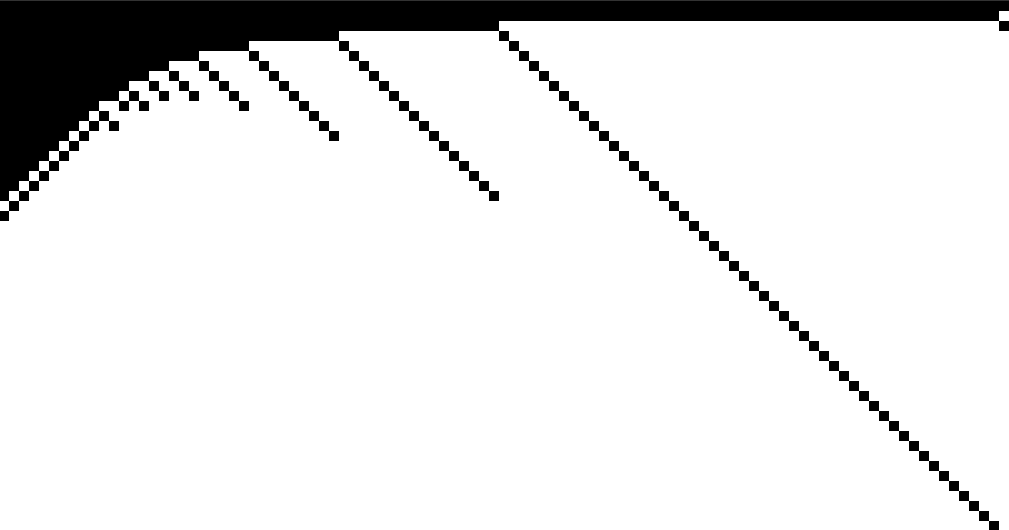
\includegraphics[width = 0.5\textwidth]{Figures/sizetwo_dim100_enlarged.png}}
		\caption{The parallel toppling odometer for $s_0 \equiv 2 d + (d-1)$ when $d = 100$ and $M=2$. A black pixel in row $t$ and column $x$ indicates that $v_t(x) = v_{t-1}(x) + 1$.  The top row is $t = 0$ and $t$ increases from top to bottom. The left column is $x = 1$ and $x$ increases from left to right. }
		\label{fig:sizetwo_dim_1_odometer}
	\end{figure}
	
	See Figure \ref{fig:sizetwo_dim_1_odometer} for a display of the odometer throughout the parallel toppling process when $s^{(d)}_0 \equiv 2d + (d-1)$ in dimension $d=100$. Visually, a contiguous block of decreasing size fires at each step, followed by a ripple of outwards firings. For $t > t_d := (\lceil \sqrt{d-1} \rceil+1)$, the firing block appears to decreases by one every step. In particular, if $a_t$ indexes the right edge of the block at time $t$, then
	$a_0=a_1=d$ and
	\[
	a_t =
	\begin{cases}
	\lfloor \frac{ d - 1}{t-1} \rfloor & \mbox{ for $t \leq t_d$ } \\
	a_{t-1} - 1 &\mbox{ for $t > t_d $}.
	\end{cases}
	\]
	This leads to a simple formula for $v_t$. %and $s_t$ when $s_0 = 2 d + (d-1)$.  
	
	\begin{prop} \label{prop:base_case}
		For all $d \geq 1$, when $s_0^{(d)} = 2 d + (d-1)$,  the radially reparameterized parallel toppling odometer has the following form. For all $t \geq 1$,
		\begin{equation} \label{eq:continuous_block}
		v_t(x) =
		\begin{cases}
		v_{t-1}(x) + 1  &\mbox{ for $x \leq a_{t}$} \\
		v_{t-1}(x)  &\mbox{ for $a_{t} < x \leq a_{t-1}$}.
		\end{cases} 
		\end{equation}
		And for each $1\leq t'<t\leq t'+x$ and $a_{t'-1}\geq x>a_{t'}$,
        \begin{equation}\label{eq:ripple}
        v_t(x)=v_{t'}(x-(t-t')).
		%v_{t}(x) = v_{t-1}(x) + (v_{t-1}(x-1)-v_{t-1}(x))
		\end{equation}
		
		
		%\begin{equation}
		%\begin{aligned}
		%v_{t-1}(x) &= v_{t-1}(x + 1) + 1 \\
		%& \implies \\
		%v_{t}(x) &= v_{t}(x+1),
		%\end{aligned}
		%\end{equation}
		
	\end{prop}
	
	\begin{proof}
        We use the radial Laplacian of Lemma~\ref{radial_laplacian}. Since $s_0\equiv 2d+(d-1)$, the height of a radial site $x$ at time $t$ is
        \begin{equation*}
        s_t(x)=2d+(d-1)+\Delta v_t(x)\,,
        \end{equation*}
        and $x$ topples at step $t+1$ exactly when $s_t(x)\geq 2d$, in which case $v_{t+1}(x)=v_t(x)+1$. Step 1 and Step 2 prove \eqref{eq:continuous_block}: for $x\leq a_t$, Step 1 at times $t$ and $t-1$ gives $v_t(x)=v_{t-1}(x)+1$, since $a_t\leq a_{t-1}$ (for $t=1$ use $v_0\equiv 0$). Step 3 proves \eqref{eq:ripple}.

        We use four facts about the edges. By definition,
        \begin{equation*}
        a_0=a_1=d\,,\qquad a_u=\Big\lfloor\frac{d-1}{u-1}\Big\rfloor\ \text{ for } 2\leq u\leq t_d\,,\qquad a_u=a_{u-1}-1\ \text{ for } u>t_d\,.
        \end{equation*}

        (F0) The edges strictly decrease: $a_{u+1}<a_u$ for $u\geq 1$. For $u\geq t_d$ this is the last case of the definition. For $u=1$ with $u+1\leq t_d$ it reads $a_2=d-1<d=a_1$. Let $u\geq 2$ with $u+1\leq t_d$, and suppose $a_{u+1}\geq a_u=:A$. Then $Au\leq a_{u+1}u\leq d-1<(A+1)(u-1)$, so $A\leq u-2$ and hence $d-1<(u-1)^2$. But $u-1<\sqrt{d-1}$, because $u\leq t_d-1=\lceil\sqrt{d-1}\rceil$. This is a contradiction.

        (F0$'$) If $a_{u-1}-a_u\geq 2$, then $u\leq t_d$, because $a_u=a_{u-1}-1$ for $u>t_d$.

        (F1) If $x\leq a_u$, then $x(u-1)\leq d-1$. For $u=1$ this reads $0\leq d-1$, and for $2\leq u\leq t_d$ it follows from $a_u\leq\frac{d-1}{u-1}$. Let $u>t_d$. If $d=1$, then $a_u\leq 0$, so $x=0$. For $d\geq 2$ put $m=t_d-1=\lceil\sqrt{d-1}\rceil$ and $r=u-t_d\geq 1$. Then $u-1=m+r$, $m^2\geq d-1$, and $a_u=a_{t_d}-r\leq\frac{d-1}{m}-r$, so
        \begin{equation*}
        x(u-1)\leq a_u(u-1)\leq\Big(\frac{d-1}{m}-r\Big)(m+r)=(d-1)+r\Big(\frac{d-1}{m}-m\Big)-r^2\leq d-1\,.
        \end{equation*}

        (F2) If $2\leq u\leq t_d$ and $a_u<x$, then $x(u-1)>d-1$, since $a_u+1>\frac{d-1}{u-1}$ and $x\geq a_u+1$.

        \emph{Step 1.} We show that $v_t(x)=t$ for every $x\leq a_t$. We induct on $t$. For $t=1$ every height at time $0$ equals $s_0\geq 2d$, so every site topples at step $1$, and $a_1=d$. Let $n\geq 1$ and assume the claim at time $n$. Let $x\leq a_{n+1}$. Since $a_{n+1}<a_n$, the sites $x-1$, $x$ and $x+1$ are all at most $a_n$, so their values at time $n$ equal $n$. (If $x=0$, the term $x\,v_n(x-1)$ vanishes.) Hence $\Delta v_n(x)=-(d+x)n+(d-x)n+xn=-xn$ and $s_n(x)=2d+(d-1)-xn$. By (F1) with $u=n+1$, $xn\leq d-1$, so $s_n(x)\geq 2d$. Thus $x$ topples at step $n+1$, and $v_{n+1}(x)=n+1$.

        \emph{Step 2.} We show that $v_{t+1}(x)=v_t(x)$ for $a_{t+1}<x\leq a_t$. Since $x$ topples at step $t+1$ exactly when $s_t(x)\geq 2d$, it suffices to show $s_t(x)<2d$. We induct on $t$, and fix $t\geq 1$ and $x$ with $a_{t+1}<x\leq a_t$.

        Case (a): $x<a_t$. Then $x-1$, $x$ and $x+1$ are at most $a_t$, so their values at time $t$ are $t$ by Step 1. Hence $\Delta v_t(x)=-xt$ and $s_t(x)=2d+(d-1)-xt$. Since $a_{t+1}<x<a_t$, the gap $a_t-a_{t+1}\geq 2$ gives $t+1\leq t_d$ by (F0$'$). Then (F2) with $u=t+1$ gives $xt>d-1$, so $s_t(x)<2d$.

        Case (b): $x=a_t$. If $t=1$, then $x=d$. The term $(d-x)v_1(x+1)$ vanishes, and $\Delta v_1(d)=-2d+d=-d$ because $v_1(d)=v_1(d-1)=1$. So $s_1(d)=2d-1$. If $t\geq 2$, then $x<d$, since $a_t\leq a_2=d-1$. Also $a_t<x+1\leq a_{t-1}$, so $v_t(x+1)=v_{t-1}(x+1)=t-1$ by the case $t-1$ of this step and by Step 1. Also $v_t(x-1)=v_t(x)=t$ by Step 1. Hence $\Delta v_t(x)=-(d+x)t+(d-x)(t-1)+xt=-xt-(d-x)$, and $s_t(x)=2d-1-(t-1)x<2d$.

        In both cases $s_t(x)<2d$, so $v_{t+1}(x)=v_t(x)$.

        \emph{Step 3.} We show \eqref{eq:ripple}. Put $k=t-t'$, so $1\leq k\leq x$, and fix $x$ with $a_{t'}<x\leq a_{t'-1}$. We induct on $k$, and for fixed $k$ on $t'$. The induction hypothesis is \eqref{eq:ripple} for every smaller shift at every front, and for the shift $k$ at every smaller front. For $k=1$ the first part is empty.

        Three values at time $t-1$ are needed.

        First, if $a_{t'}<z\leq a_{t'-1}$ and $z\geq k-1$, then $v_{t-1}(z)=t'$ when $z-k+1\leq a_{t'}$, and $v_{t-1}(z)=t'-1$ otherwise. Indeed $v_{t-1}(z)=v_{t'}(z-k+1)$ by the hypothesis for shift $k-1$ at front $t'$, which is trivial when $k=1$. Steps 1 and 2 give the values of $v_{t'}$: it equals $t'$ on $\{w\leq a_{t'}\}$ and $t'-1$ on $\{a_{t'}<w\leq a_{t'-1}\}$.

        Second, $v_{t-1}(a_{t'})\in\{t',t'+1\}$. For $k=1$ this is $v_{t'}(a_{t'})=t'$ by Step 1. For $k\geq 2$, the site $a_{t'}$ lies in the window of front $t'+1$, so the hypothesis for shift $k-2$ at front $t'+1$ gives $v_{t-1}(a_{t'})=v_{t'+1}(a_{t'}-k+2)$. Steps 1 and 2 at time $t'+1$ show that this value is $t'$ or $t'+1$.

        Third, if $x=a_{t'-1}<d$, then $v_{t-1}(x+1)=t'-1$. The site $x+1$ lies in the window of front $t'-1$, so the hypothesis for shift $k$ at front $t'-1$ gives $v_{t-1}(x+1)=v_{t'-1}(x+1-k)$. Since $x+1-k\leq a_{t'-1}$, Step 1 makes this $t'-1$.

        Write $\lambda=v_{t-1}(x-1)$, $\beta=v_{t-1}(x)$ and $\rho=v_{t-1}(x+1)$. The radial Laplacian gives
        \begin{equation*}
        s_{t-1}(x)-2d=(d-1)-(d+x)\beta+(d-x)\rho+x\lambda\,.
        \end{equation*}
        If $x=d$, then the term $(d-x)\rho$ vanishes, and we set $\rho=t'-1$ in that case; the third fact is then not needed.

        We split by the position of $x-k$ relative to $a_{t'}$. In each case we show $v_t(x)=v_{t'}(x-k)$. By Steps 1 and 2 this value is $t'$ when $x-k\leq a_{t'}$, and $t'-1$ when $x-k>a_{t'}$.

        \emph{Behind,} $x-k<a_{t'}$. Here $\beta=t'$ by the first fact, since $x-k+1\leq a_{t'}$. By the first and second facts, $\lambda=t'+\alpha$ with $\alpha\in\{0,1\}$. By the first and third facts, $\rho=t'-\gamma$ with $\gamma\in\{0,1\}$. Then
        \begin{equation*}
        s_{t-1}(x)-2d=(d-1)-xt'+x\alpha-(d-x)\gamma\,.
        \end{equation*}
        If $\gamma=1$, then this equals $-1-x(t'-1)+x\alpha\leq -1-x(t'-2)<0$, because $\alpha\leq 1$ and $t'\geq 2$. If $\gamma=0$, then $\rho=t'$ forces $x+1\leq a_{t'-1}$. So $a_{t'-1}-a_{t'}\geq 2$, and $t'\leq t_d$ by (F0$'$). Since $a_{t'}<x$, (F2) with $u=t'$ gives $x(t'-1)>d-1$. Then $s_{t-1}(x)-2d=(d-1)-x(t'-1)-x(1-\alpha)<0$. In both cases $s_{t-1}(x)<2d$, so $x$ does not topple at step $t$, and $v_t(x)=\beta=t'$.

        \emph{At the front,} $x-k=a_{t'}$. Here $\beta=t'-1$ by the first fact, since $x-k+1=a_{t'}+1$. The value $\lambda$ equals $t'$. For $k\geq 2$ this is the first fact, since $x-1$ lies in the window and $(x-1)-k+1=a_{t'}$. For $k=1$ it holds because $x-1=a_{t'}$ and $t-1=t'$. The value $\rho$ equals $t'-1$ by the first or third fact, since $(x+1)-k+1=a_{t'}+2$. Hence
        \begin{equation*}
        s_{t-1}(x)-2d=(d-1)+(2-t')x=(d-1)-x(t'-2)\,.
        \end{equation*}
        Since $x\leq a_{t'-1}$, (F1) with $u=t'-1$ gives $x(t'-2)\leq d-1$. So $s_{t-1}(x)\geq 2d$, $x$ topples at step $t$, and $v_t(x)=t'=v_{t'}(x-k)$.

        \emph{Ahead,} $x-k>a_{t'}$. Then $x-1\geq x-k>a_{t'}$, and the first and third facts give $\lambda=\beta=\rho=t'-1$. Hence $s_{t-1}(x)-2d=(d-1)-x(t'-1)$. Since $x\geq (x-k)+1\geq a_{t'}+2$ and $x\leq a_{t'-1}$, we have $a_{t'-1}-a_{t'}\geq 2$, so $t'\leq t_d$ by (F0$'$). Then (F2) with $u=t'$ gives $x(t'-1)>d-1$. So $s_{t-1}(x)<2d$, $x$ does not topple at step $t$, and $v_t(x)=t'-1=v_{t'}(x-k)$.

        In all three cases $v_t(x)=v_{t'}(x-k)$, which is \eqref{eq:ripple}.
    \end{proof}
	
	
	
	\section{Odometer regularity when \texorpdfstring{$d = 1$}{d=1}} \label{sec:base_regularity}
		From here onward, suppose $s_0 \equiv 2 d$. We start the inductive proof of Theorem \ref{the_theorem} by establishing some regularity of the odometer in the critical dimension $d=d_0=1$.   In the next section, we inductively use dimensional reduction to show that $d \geq 2$ sandpiles inherit this regularity. This regularity ensures that the dynamics of lower-dimensional sandpiles agree with their higher-dimensional embeddings. 
		
		When reading Section \ref{sec:dim_reduction} below, the reader should observe that whenever Proposition \ref{base_dimension} (or something close to it) holds, dimensional reduction 
		follows. For example, if a version of this result is established in every critical dimension $d_0 \geq 1$,  
		then dimensional reduction follows for all sandpiles of the form $2 d + (d_0 - 1)$ in dimensions $d > d_0$. 
		Proposition \ref{prop:base_case} should be understood as a step in this direction. 


	
	
	
	\begin{prop}\label{base_dimension}
		Recall the definition of $\tau_{j}$ from Theorem \ref{the_theorem}. For all $M \geq 2$ and $d \geq 1$, the odometer maintains the following properties throughout the parallel toppling process.
		\begin{description}
			\item[Self-similarity]  For each $1 \leq j \leq M$ and $t \leq \tau_j$ 
			\begin{equation} \label{base_dimension:consistency}
			v_t^{(M)}(\mathbf{x}) =  v_t^{(j)}(\mathbf{x}-(M-j))  \mbox{ for $\mathbf{x} > M-j$}.
			\end{equation}
			\item[Weak facet compatibility] For all $\mathbf{x}_i \geq 2$, $t \geq 1$, $i \geq 0$, $j \geq 0$ and $i+j+1=d$
			\begin{equation} \label{base_dimension:weak_compatability}
			\begin{aligned}
			v_t^{(M)}(\mathbf{x}_i, 1, \mathbf{1}_j) &= v_t^{(M)}(\mathbf{x}_i, 2, \mathbf{1}_j)+ 1  \\
			& \implies \\
			v_{t+1}^{(M)}(\mathbf{x}_i,1,\mathbf{1}_j)
            &=v_t^{(M)}(\mathbf{x}_i,1,\mathbf{1}_j).
			\end{aligned} 
			\end{equation}
			\item[Strong facet compatibility] Let $i,j\geq0$, $i+1+j=d$,
            and put $p=(\mathbf{x}_i,1,\mathbf{1}_j)\in\mathcal S_M^{(d)}$
            with $\mathbf{x}_i\geq2$. If $t<\tau_M$, or if $i\geq1$ and
            $t\geq\tau_M$, then
            \begin{equation}\label{base_dimension:strong_derivative}
            v_t^{(M)}(p)-v_t^{(M)}(p+2e_{i+1})\leq2
			\end{equation}
			and
			\begin{equation} \label{base_dimension:strong_compatability}
			\begin{aligned} 
			v_t^{(M)}(\mathbf{x}_i,1,\mathbf{1}_j)
            &=v_t^{(M)}(\mathbf{x}_i,2,\mathbf{1}_j)+1\\
			& \implies \\
			v_{t+1}^{(M)}(\mathbf{x}_i, 1, \mathbf{1}_j) &= v_{t}^{(M)}(\mathbf{x}_i, 1, \mathbf{1}_j) \\
			v_{t+1}^{(M)}(\mathbf{x}_i, 2, \mathbf{1}_j) &= v_{t}^{(M)}(\mathbf{x}_i, 2, \mathbf{1}_j)+1.
			\end{aligned}
			\end{equation}

		
			
			\item[Strong topple control] 
			For all $t \geq \tau_{M-1}$, 
			\begin{equation} \label{base_dimension:strong_topple}
			\sup_{\mathbf{x} \in \mathcal{S}_M} \left(v_{t+2}(\mathbf{x}) - v_{t}(\mathbf{x})\right) \leq 1.
			\end{equation}

			
		\end{description}
		
	\end{prop}
	
	\begin{proof}[Proof of Proposition \ref{base_dimension} for $d=d_0 = 1$]
		The proof proceeds by induction on $M$ and then on $t$. When $M=2$, 
		\begin{center}
			\begin{tabular}{l|l|l}
				& $v_t^{(M)}(1)$ & $v_t^{(M)}(2)$ \\ \hline
				$t=1$ & 1 & 1  \\ 
				$t=2$ & 2 & 1  \\ 
				$t=3$ & 2 & 2 \\
				$t=4$ & 3 & 2 
			\end{tabular}
		\end{center}
		and $v_1^{(M-1)}(1) = v_2^{(M-1)}(1) = 1$ which verifies the base case. Now, let $M$ be given and note that
		$v_1^{(M)}(x) = 1$ for all $1 \leq x \leq M$ and $v_2^{(M)}(x) = 2$ for $1 \leq x < M$
		and $v_2^{(M)}(M) = 1$. Hence, suppose \eqref{base_dimension:consistency},\eqref{base_dimension:weak_compatability},\eqref{base_dimension:strong_derivative},\eqref{base_dimension:strong_compatability}, hold for $(M-1)$ for all $t \geq 1$ 
		and suppose they hold for $M$ for all $t' \leq (t-1)$. 
		We verify each inductive step. 
		
		\subsubsection*{Self-similarity: \eqref{base_dimension:consistency}}
		By strong induction, it suffices to show $v_t^{(M)}(x) = v_t^{(M-1)}(x-1)$ for $x \geq 2$.
		By Lemma \ref{pt_ind_lemma}, 
		\[
		v_{t}^{(M)}(x) = 1 + \lfloor \frac{v_{t-1}^{(M)}(x+1) + v_{t-1}^{(M)}(x-1)}{2} \rfloor
		\]
		for $x > 1$. 
		Hence, by \eqref{base_dimension:consistency} at $(t-1)$, for $x > 2$, 
		\[
		v_{t}^{(M)}(x) = 1 + \lfloor \frac{v_{t-1}^{(M-1)}(x) + v_{t-1}^{(M-1)}(x-2)}{2} \rfloor = v_t^{(M-1)}(x-1).
		\]
		For $x=1$, we have reflection at the origin, 
		\[
		v_{t}^{(M-1)}(1) = 1 + \lfloor \frac{v_{t-1}^{(M-1)}(2) + v_{t-1}^{(M-1)}(1)}{2} \rfloor = 1 + \lfloor \frac{v_{t-1}^{(M)}(3) + v_{t-1}^{(M)}(2)}{2} \rfloor.
		\]
		Hence, if $v_{t-1}^{(M)}(1) = v_{t-1}^{(M)}(2)$, then $v_{t}^{(M-1)}(1) = v_{t}^{(M)}(2)$. 
		
		When $v_{t-1}^{(M)}(1) = v_{t-1}^{(M)}(2) + 1$, we instead use strong facet compatibility 
		in both layers. If $v_{t-1}^{(M-1)}(1) = v_{t-1}^{(M-1)}(2)$, then $v_{t}^{(M-1)}(1) = v_{t-1}^{(M-1)}(1) + 1$ and we are done, so suppose not. Since sites topple at most once per time step by Lemma \ref{topple_limit}, 
		the odometer must then be,  for some $v \geq 2$:
		\begin{center}
			\begin{tabular}{l | l | l | l }
				& $v_{\cdot}^{(M)}(1)$ & $v_{\cdot}^{(M)}(2)$ & $v_{\cdot}^{(M)}(3)$ \\  \hline
				$t-2$ & $v$ & $v$ & $v-1$    \\
				$t-1$  & $v+1$ & $v$  & $v-1$  \\   
				$t$  & $v+1$ & $v+1$ & $\geq (v-1)$
			\end{tabular}
		\end{center}
		This contradicts strong facet compatibility for $v_t^{(M-1)}(1)$ from $(t-2) \to (t-1)$, which 
		we can use as $t \leq \tau_{M-1}$ and hence $(t-1) < \tau_{M-1}$.
		
		\subsubsection*{Weak facet compatibility: \eqref{base_dimension:weak_compatability}}
		% This is especially simple in one dimension. 
		If $v_t(1) = v_t(2) + 1$, then $\Delta v_t(1) = -1$ and so $v_{t+1}(1) = v_{t}(1)$. 
		
		%In higher dimensions, as facets consist of more than one point, the proof of this requires analysis of a burn-in %phase, which we carry out in the next section. .
		
		
		
		
		\subsubsection*{Strong facet compatibility: \eqref{base_dimension:strong_derivative} and \eqref{base_dimension:strong_compatability}} 
		
		We use Lemma \ref{general_difference_comparison} to show \eqref{base_dimension:strong_derivative}.
		The function $g(x) = 2 x$ is harmonic in the interior of the interval so it suffices to check 
		the dissipating and reflecting boundaries. We control the dissipating boundary using $t < \tau_M$
		and the reflecting boundary with \eqref{base_dimension:weak_compatability}. 
		
		As $t < \tau_M$, $v_t(M) \leq (M-1)$ and hence by Corollary \ref{cor:derivative_bound}, 
		$v_t(M-1) \leq v_{t}(M) + (M-1) \leq 2 (M-1)$. For the reflecting boundary, i.e, $x=1$, we check  
		\begin{align*}
		\sum_{y \sim x} v_t(y) - \sum_{y' \sim (x+2)} v_t(y) &= (v_t(1) - v_t(2)) + (v_t(2) - v_t(4))  \leq (v_t(1) - v_t(2)) + 4.
		\end{align*}
		If $v_t(1) - v_t(2) = 1$, then $v_{t+1}(1) = v_{t}(1)$ by weak facet compatibility. 
		Otherwise, $\sum_{y \sim x} v_t(y) - \sum_{y' \sim (x+2)} v_t(y) \leq 4$ and we conclude that 
		\[
		v_t(x) - v_t(x + 2) \leq 2 x. 
		\]
		Taking $x=1$, this implies 
		\[
		\Delta v_t(2) \geq -2 v_t(2) + v_t(1) + v_t(1) -2
		\geq 0, 
		\]
		which shows \eqref{base_dimension:strong_compatability}. 
		
		\subsubsection*{Strong topple control: \eqref{base_dimension:strong_topple}}
		By Lemma \ref{topple_limit}, it suffices to show 
		\[ 
		\sup_{x \in \mathcal{S}_M} \left(v_{\tau_{M-1}+2}(x) - v_{\tau_{M-1}}(x)\right) \leq 1
		\]
		First observe that \eqref{base_dimension:consistency} for $v_t^{(M)}$ and \eqref{base_dimension:strong_topple} for $v_t^{(M-1)}$ imply that
		\begin{equation} \label{eq:topple_time_lower_bound}
		\tau_{M-1} \geq \tau_{M-2} + 2. 
		\end{equation}
		Suppose for sake of contradiction that 
		\[
		\left(v_{\tau_{M-1}+2}(x) - v_{\tau_{M-1}}(x)\right) = 2
		\]
		for some $1 \leq x \leq M$. Lemma \ref{topple_limit} then implies
		that some neighbor $y \sim x$ must have toppled twice previously. Pick 
		the maximal such $y$.  We consider three cases for $y$. 
		
		{\bf Case 1: $y \geq 3$} \\
		We first note that $v_{\tau_{M-1}+1}^{(M)}(y) = v_{\tau_{M-1}+1}^{(M-1)}(y-1)$.
		Indeed, by \eqref{base_dimension:consistency}, as $(y-1) \geq 2$, 
		\begin{align*}
		v_{\tau_{M-1}+1}^{(M)}(y) &= 1 + \lfloor \frac{v_{\tau_{M-1}}^{(M)}(y+1) + v_{\tau_{M-1}}^{(M)}(y-1)}{2} \rfloor  \\
		&= 1 + \lfloor \frac{v_{\tau_{M-1}}^{(M-1)}(y) + v_{\tau_{M-1}}^{(M-1)}(y-2)}{2} \rfloor  \\
		&= 	v_{\tau_{M-1}+1}^{(M-1)}(y-1)
		\end{align*}
		Hence, 	
		\[
		2 = v_{\tau_{M-1}+1}^{(M)}(y)-v_{\tau_{M-1}-1}^{(M)}(y) = v_{\tau_{M-1}+1}^{(M-1)}(y-1)-v_{\tau_{M-1}-1}^{(M-1)}(y-1),
		\]
		which contradicts \eqref{base_dimension:strong_topple} for $v_t^{(M-1)}$.
		
		
		{\bf Case 2: $y = 2$} \\
		We claim that $v_{\tau_{M-1}+1}^{(M)}(2) = v_{\tau_{M-1}+1}^{(M-1)}(1)$, in which 
		case we can use the argument of Case 1. If not, then $v_{\tau_{M-1}}^{(M)}(2) = v_{\tau_{M-1}}^{(M)}(3)+1$
		but $v_{\tau_{M-1}}^{(M)}(1) = v_{\tau_{M-1}}^{(M)}(2)+1$. This implies that either 
		\[
		v_{\tau_{M-1}-1}^{(M)}(1) = v_{\tau_{M-1}-1}^{(M)}(2)+2
		\]
		or
		\begin{align*}
		v_{\tau_{M-1}-1}^{(M)}(1) &= v_{\tau_{M-1}-1}^{(M)}(2)+1 \\
		 &\mbox{ and }  \\  
		v_{\tau_{M-1}}^{(M)}(1) &= v_{\tau_{M-1}-1}^{(M)}(1)+1
		\end{align*}
		both which contradict weak facet compatibility. 


		{\bf Case 3: $y = 1$} \\
		In this case, the odometer near the center must be, for some $v \geq 1$,
			\begin{center}
			\begin{tabular}{l | l | l | l }
				& $v_{\cdot}^{(M)}(1)$ & $v_{\cdot}^{(M)}(2)$ & $v_{\cdot}^{(M)}(3)$ \\  \hline
				$\tau_{M-1}-1$ & $v$ & $v$ & $v$    \\
				$\tau_{M-1}$  & $v+1$ & $v+1$  & $v$  \\   
				$\tau_{M-1}+1$  & $v+2$ & $v+1$ & $\geq (v)$
			\end{tabular}
		\end{center}
		This shows $v^{(M)}_{\tau_{M-1}-2}(2) = v-1$. Indeed, 
		if $v^{(M)}_{\tau_{M-1}-2}(1) = v-1$, then as $\Delta v^{(M)}_{\tau_{M-1}-2}(1) \geq 0$
		 $v^{(M)}_{\tau_{M-1}-2}(2) = v-1$. If $v^{(M)}_{\tau_{M-1}-2}(1) = v$, then $\Delta v^{(M)}_{\tau_{M-1}-2}(1) \leq -1$ and $v^{(M)}_{\tau_{M-1}-2}(2) = v-1$. Hence, 
		 \[
		 v^{(M-1)}_{\tau_{M-1}}(1) = v^{(M)}_{\tau_{M-1}}(2) = v^{(M)}_{\tau_{M-1}-2}(2)+2= v^{(M-1)}_{\tau_{M-1}-2}(2)+2,
		 \]
		 which contradicts \eqref{base_dimension:strong_topple} for $v_t^{(M-1)}$ using \eqref{eq:topple_time_lower_bound}.


	\end{proof}
	
	\begin{lemma}\label{lem:one-terminal-profile}
    In dimension one, with $s_0\equiv2$ and $1\leq x\leq M$,
    \[
    v_\infty(x)=\frac{M(M+1)-x(x-1)}2,\qquad
    v_\infty(x)-v_\infty(x+1)=x,
    \]
    where $v_\infty(M+1)=0$ is the dissipating boundary value.
    \end{lemma}
    \begin{proof}
    The formula $Q(x)=\frac{M(M+1)-x(x-1)}{2}$ defines an integer valued function on $\mathbb{Z}$, since $M(M+1)$ and $x(x-1)$ are even. For every integer $x$,
    \begin{equation*}
    Q(1-x)=Q(x)\,,\qquad Q(x)-Q(x+1)=x\,.
    \end{equation*}
    Hence $Q(0)=Q(1)$ and $Q(M+1)=0$. Also $\Delta Q(x)=(Q(x+1)-Q(x))+(Q(x-1)-Q(x))=-x+(x-1)=-1$ for every $x$. Since $Q$ decreases on $\{1,\dots,M+1\}$ to $Q(M+1)=0$, it is nonnegative on $\{1,\dots,M\}$, and by the symmetry $Q(1-x)=Q(x)$ also on $\{1-M,\dots,0\}$.

    \emph{Step 1.} We show that $v_t\leq Q$ on the cube $\{1-M,\dots,M\}$ for every $t$. The function $Q$ is nonnegative and integer valued there, and $\Delta Q+s_0=-1+2=1=2d-1$ (here $d=1$). So $Q$ stabilizes $s_0$, and the parabolic least action principle (Lemma~\ref{parabolic_comparison}) gives $v_t\leq Q$ for every $t$.

    \emph{Step 2.} We show that the odometer stops changing. Each $v_t(x)$ is nondecreasing in $t$ and bounded by $Q(x)$ by Step 1, so it is eventually constant. The cube is finite, so there is a time $T$ with $v_{T+1}=v_T$, and then $v_\infty=v_T$.

    \emph{Step 3.} We show that $v_T\geq Q$ on $\{1,\dots,M\}$. Since no site topples at step $T+1$, the sandpile $s_T=2+\Delta v_T$ is at most $1$ on $\{1,\dots,M\}$, so $\Delta v_T\leq -1$ there. Put $q=v_T-Q$. Then $\Delta q\leq 0$ on $\{1,\dots,M\}$. Let $\rho_x=q(x+1)-q(x)$. Then $\Delta q(x)=\rho_x-\rho_{x-1}$, so $\rho_x\leq\rho_{x-1}$ for $1\leq x\leq M$. The odometer is symmetric under $x\mapsto 1-x$ (Section~\ref{subsec:symmetry}), and so is $Q$, so $q(0)=q(1)$, that is, $\rho_0=0$. Hence $\rho_x\leq 0$ for $0\leq x\leq M$, and $q$ is nonincreasing on $\{1,\dots,M+1\}$. Both $v_T$ and $Q$ vanish at $M+1$, so $q(M+1)=0$, and therefore $q\geq 0$ on $\{1,\dots,M\}$.

    \emph{Step 4.} By Steps 1 to 3, $v_\infty=v_T=Q$ on $\{1,\dots,M\}$, which is the displayed formula. Since $v_\infty(M+1)=0=Q(M+1)$, the identity $Q(x)-Q(x+1)=x$ gives $v_\infty(x)-v_\infty(x+1)=x$ for $1\leq x\leq M$, including $x=M$.
    \end{proof}
    Hence the restriction $t<\tau_M$ is needed for strong facet compatibility
    when the head is empty.
	
	\section{Odometer regularity and dimensional reduction} \label{sec:dim_reduction}
	We now prove Proposition \ref{base_dimension} for $d \geq 2$ together with dimensional reduction,
	\begin{equation} \label{eq:reduction_gen_d}
	v_t^{(d,M)}(\mathbf{x}_{d-1},1) = v_{t}^{(d-1,M)}(\mathbf{x}_{d-1}),
	\end{equation}
	 by strong induction on $M$, $d$, and $t$. Specifically, given $M$, $d$, and $t$, suppose
	 \[ \eqref{base_dimension:consistency},\eqref{base_dimension:weak_compatability},\eqref{base_dimension:strong_derivative},\eqref{base_dimension:strong_compatability}, \eqref{base_dimension:strong_topple}
	 \]
	 hold for
	\begin{align*}
	v_{t'}^{(d', M')} &\quad \mbox{for all $M' \geq 1$, $t' \geq 1$, $d' < d$}, \\
	v_{t'}^{(d, M')} &\quad \mbox{for all $M' < M$, $t' \geq 1$}, \\
	v_{t'}^{(d, M)} &\quad \mbox{for all $t' < t$}.
	\end{align*}
	We also suppose  \eqref{eq:reduction_gen_d} holds for $v_{t-1}^{(d',M')}$ for all $d' \geq 2$ and $M' \leq M$.
	Indeed, $v_{1}^{(d,M)} \equiv 1$ for all $d \geq 1$ and $M \geq 1$.

	\subsection{Dimensional reduction}
	We start the induction in time by proving dimensional reduction given odometer regularity at $(t-1)$. 
	Let $\mathbf{x}_{d-1}$ be given and pick the smallest $d > i \geq 0$ so that
	$(\mathbf{x}_i, \mathbf{1}_{d-i}) = (\mathbf{x}_{d-1},1)$. 
	By symmetry, 
	\begin{align}
	\notag  \Delta^{(d)} v_{t-1}^{(d)}(\mathbf{x}_{i}, \mathbf{1}_{d-i}) &= -2 d v_{t-1}^{(d)}(\mathbf{x}_{i}, \mathbf{1}_{d-i}) \\  
	\notag  &+  \sum_{\mathbf{y}_{i} \sim \mathbf{x}_{i}} v_{t-1}^{(d)}(\mathbf{y}_{i}, \mathbf{1}_{d-i}) \\
	\notag  &+ (d-i) \left( v_{t-1}^{(d)}(\mathbf{x}_{i}, \mathbf{1}_{d-i})   + v_{t-1}^{(d)}(\mathbf{x}_{i},2, \mathbf{1}_{d-i-1})  \right).
	\end{align}
	
	We consider two cases at time $(t-1)$. 
	
	
	{\bf Case 1}: $v_{t-1}^{(d)}(\mathbf{x}_{i}, \mathbf{1}_{d-i}) = v_{t-1}^{(d)}(\mathbf{x}_{i},2, \mathbf{1}_{d-i-1})$
	
	 By \eqref{eq:reduction_gen_d} at $(t-1)$, $v_{t-1}^{(d)}(\mathbf{x}_i, \mathbf{1}_{d-i}) = v_{t-1}^{(i+1)}(\mathbf{x}_{i},1)$.
	Thus,
	\begin{align*}
	\Delta^{(d)} v_{t-1}^{(d,M)}(\mathbf{x}_{i}, \mathbf{1}_{d-i}) &= -2 i v_{t-1}^{(i+1)}(\mathbf{x}_{i},1) +  \sum_{\mathbf{y}_{i} \sim \mathbf{x}_{i}} v_{t-1}^{(i+1)}(\mathbf{y}_{i},1)  \\
	&=  \Delta^{(i+1)} v_{t-1}^{(i+1,M)}(\mathbf{x}_{i},1)
	\end{align*}
	which concludes this case as $v_{t}^{(d)} = v_{t-1}^{(d)} + 1(\Delta^{(d)} v_{t-1}^{(d)} \geq 0)$. 	

	
	{\bf Case 2: $v_{t-1}^{(d)}(\mathbf{x}_{i}, \mathbf{1}_{d-i}) = v_{t-1}^{(d)}(\mathbf{x}_{i},2, \mathbf{1}_{d-i-1}) + 1$} \\
	If $i \leq (d-2)$, then \eqref{base_dimension:weak_compatability} for $(t-1) \to t$
	for both $v_{t-1}^{(i+1)}$ and $v_{t-1}^{(d)}$ imply that 
	\[
	v_{t-1}^{(i+1)}(\mathbf{x}_i,1) = v_{t-1}^{(d)}(\mathbf{x}_{i}, \mathbf{1}_{d-i})  = v_{t}^{(d)}(\mathbf{x}_{i}, \mathbf{1}_{d-i}) = v_{t}^{(i+1)}(\mathbf{x}_i,1).
	\]
	If $i = (d-1)$, then \eqref{base_dimension:strong_compatability} and \eqref{eq:reduction_gen_d} at $(t-1)$ and $(t-2)$ imply that 
	\[
	v_{t-1}^{(d-1)}(\mathbf{x}_{d-1}) = v_{t-1}^{(d)}(\mathbf{x}_{d-1},1) = v_{t-2}^{(d)}(\mathbf{x}_{d-1},1)+1 = 
	v_{t-2}^{(d-1)}(\mathbf{x}_{d-1})+1.
	\]	
	If $(t-2) \geq \tau_{M-1}$, \eqref{base_dimension:strong_topple} for $v_t^{(i)}$ and $v_t^{(d)}$  imply that
	\[
	v_{t}^{(d-1)}(\mathbf{x}_{d-1}) =	v_{t-1}^{(d-1)}(\mathbf{x}_{d-1}) = v_{t-1}^{(d)}(\mathbf{x}_{d-1},1) = v_{t}^{(d)}(\mathbf{x}_{d-1},1).
	\]
	If $(t-2) < \tau_{M-1}$, then \eqref{base_dimension:consistency} and \eqref{eq:reduction_gen_d} for $v_{t-1}^{(M-1)}$ show
	\[
	v_{t-1}^{(d,M)}(\mathbf{x}_{d-1},2) = v_{t-1}^{(d,M-1)}(\mathbf{x}_{d-1}-1,1) = v_{t-1}^{(d-1,M-1)}(\mathbf{x}_{d-1}-1).
	\]
	Similarly, 
	\[
	v_{t-1}^{(d,M)}(\mathbf{x}_{d-1},1) = v_{t-1}^{(d-1,M)}(\mathbf{x}_{d-1}) = v_{t-1}^{(d-1,M-1)}(\mathbf{x}_{d-1}-1).
	\]
	Therefore, for all $t' \leq \tau_{M-1}$, 
	\begin{equation} \label{eq:reflecting_boundaries}
	v_{t'}^{(d,M)}(\mathbf{x}_{d-1},2) = v_{t'}^{(d,M)}(\mathbf{x}_{d-1},1),
	\end{equation}
	this however contradicts the case we are in. 

	


\subsection{Odometer regularity for \texorpdfstring{$d \geq 2$}{d >= 2}}

We verify each inductive step. 


\subsubsection*{Self-similarity: \eqref{base_dimension:consistency}}
As $\eqref{base_dimension:consistency}$ holds for $(M-1)$ at $t$, it suffices to show 
that if $t \leq \tau_{M-1}$ and $\mathbf{x} > 1$,
\begin{equation}\label{eq:self_sim1}
v_t^{(M)}(\mathbf{x}) = v_t^{(M-1)}(\mathbf{x}-1).
\end{equation}
We split verification of this into cases. 

{\bf Case 1: $\mathbf{x} > 2$} \\ 
As \eqref{eq:self_sim1} holds for $(t-1)$, by Lemma \ref{pt_ind_lemma}, 
\begin{align*}
v_{t}^{(M)}(\mathbf{x}) &= \lfloor \frac{ s_0(\mathbf{x}) + \sum_{\mathbf{y} \sim \mathbf{x}} v_{t-1}^{(M)}(\mathbf{y}) }{2 d} \rfloor \\
&= \lfloor \frac{ s_0(\mathbf{x}-1) + \sum_{\mathbf{y} \sim (\mathbf{x}-1)} v_{t-1}^{(M-1)}(\mathbf{y})}{2 d} \rfloor \\
&= v_t^{(M-1)}(\mathbf{x}-1).
\end{align*}

{\bf Case 2:  $\mathbf{x} = (\mathbf{x}_j, \mathbf{2})$ for $\mathbf{x}_j > 2$ and $0 \leq j < d$ } \\
We show that if $\Delta v_{t-1}^{(M)}(\mathbf{x}) \geq 0$, then  $\Delta v_{t-1}^{(M-1)}(\mathbf{x}-1) \geq 0$.
First, decompose the Laplacian into a sum of discrete second differences,
\[
\Delta v_{t-1}^{(M)}(\mathbf{x}) = \sum_{i=1}^d \Delta_{(i)} v_{t-1}^{(M)}(\mathbf{x}),
\]
where 
\[
\Delta_{(i)} v_{t-1}^{(M)}(\mathbf{x}) =  - 2 v_{t-1}^{(M)}(\mathbf{x}) + v_{t-1}^{(M)}(\mathbf{x}+e_i) + v_{t-1}^{(M)}(\mathbf{x}-e_i). 
\]
Observe that \eqref{base_dimension:consistency} at $(t-1)$ implies, 
$\Delta_{(i)} v_{t-1}^{(M)}(\mathbf{x}) = \Delta_{(i)} v_{t-1}^{(M-1)}(\mathbf{x}-1)$
for all $i \leq j$ and for $i > j$, 
\[
\Delta_{(i)} (v_{t-1}^{(M-1)}(\mathbf{x}-1) - v_{t-1}^{(M)}(\mathbf{x})) = v_{t-1}^{(M-1)}(\mathbf{x}-e_i-1) - v_{t-1}^{(M)}(\mathbf{x}-e_i).
\]
By reflectional symmetry, for each $i > j$, 
\[
v_{t-1}^{(M-1)}(\mathbf{x}-e_i-1) = v_{t-1}^{(M-1)}(\mathbf{x}-1) = v_{t-1}^{(M)}(\mathbf{x}),
\]
%and $v_{t-1}^{(M)}(\mathbf{x}-e_i) = v_{t-1}^{(M)}(\mathbf{x}_j, \mathbf{2}, 1)$ 
thus 
\begin{equation} \label{eq:difference}
\Delta_{(i)} (v_{t-1}^{(M-1)}(\mathbf{x}-1) - v_{t-1}^{(M)}(\mathbf{x}))  = v_{t-1}^{(M)}(\mathbf{x}) - v_{t-1}^{(M)}(\mathbf{x}-e_i).
\end{equation}
If $v_{t-1}^{(M)}(\mathbf{x}) = v_{t-1}^{(M)}(\mathbf{x}-e_i)$ for all $i > j$, we are done, so suppose otherwise.


Take $i > j$ where $\eqref{eq:difference} \not = 0$. By \eqref{base_dimension:strong_compatability}, 
\begin{equation} \label{eq:loaded_spring}
v_{t-2}^{(M)}(\mathbf{x}) =  v_{t-1}^{(M)}(\mathbf{x}) =  v_{t-1}^{(M)}(\mathbf{x}-e_i)-1 = v_{t-2}^{(M)}(\mathbf{x}-e_i).
\end{equation}
%but
%\[
%v_{t-2}^{(M)}(\mathbf{x}) = v_{t-2}^{(M)}(\mathbf{x}-e_i).
%\]
By \eqref{base_dimension:consistency} and \eqref{base_dimension:strong_compatability} for $v_{t-2}^{(M-1)}$, if
\[
v_{t-1}^{(M-1)}(\mathbf{x}-1) =  v_{t-1}^{(M-1)}(\mathbf{x}-1+e_i)+1
\]
then 
\[
v_{t-1}^{(M)}(\mathbf{x}) = v_{t-1}^{(M-1)}(\mathbf{x}-1) =  v_{t-2}^{(M-1)}(\mathbf{x}-1)+1 = v_{t-2}^{(M)}(\mathbf{x}) + 1
%v_{t-1}^{(M)}(\mathbf{x}) = v_{t-2}^{(M)}(\mathbf{x}) +1 =v_{t-2}^{(M)}(\mathbf{x}-e_i) +1
\]
which contradicts \eqref{eq:loaded_spring}. Moreover, 
by \eqref{base_dimension:strong_compatability}
we must have for each neighbor $(\mathbf{y}-e_i) \sim (\mathbf{x} - e_i)$, $v_{t-1}^{(M)}(\mathbf{y}) \geq v_{t-2}^{(M)}(\mathbf{y}-e_i)$. Thus, 
\begin{equation} 
\Delta v_{t-1}^{(M-1)}(\mathbf{x}-1) \geq  \Delta v_{t-2}^{(M)}(\mathbf{x}-e_i) \geq 0.
\end{equation}



\subsubsection*{Strong facet compatibility: \eqref{base_dimension:strong_derivative}
    and \eqref{base_dimension:strong_compatability}}
The regularity clauses and finite dimensional reduction can be proved jointly
in lexicographic order of dimension, side length and time. At a fixed triple,
prove dimensional reduction first, then the strong derivative bound, then the
two strong compatibility conclusions, followed by weak compatibility and
self-similarity, and finally strong topple control. Any regularity assertion
used to obtain the strong derivative bound is at an earlier time.
For a nonempty head, Lemma~\ref{lem:strict-head-facet} below states both the
constant-two bound and the two firing conclusions, at every time. Its closed
conclusions also follow from the completed joint induction; they must not be
fed back into that induction as additional assumptions. The independent
argument below gives an alternative proof using first waits.
For an empty head the point is $\mathbf1$ and the permitted regime is
$t<\tau_M$. Case~1 gives the constant-two bound using earlier weak
compatibility. The no-fire conclusion follows from the reflected Laplacian
at $\mathbf1$: a unit gap gives $\Delta v_t(\mathbf1)=-d$.
For the raised site's firing conclusion, compare its current neighbor sum
with the preceding neighbor sum at $\mathbf1$, using the early two-step
bound and the earlier compatibility assertions. This is the same generic
facet comparison used in the joint induction, with its exceptional early
subcases resolved by earlier dimensional reduction. No all-time raised-site
firing is claimed at $\mathbf1$.
{\bf Case 1: $t<\tau_M$} \\
We prove $v_t(x)-v_t(x+2e_k)\leq2x_k$ for every $1\leq k\leq d$ on
$P_M=\{1,\ldots,M\}^d$, by induction up to the indicated time. The first
difference is bounded by $x_k$. Before $\tau_M$, every physical inner-boundary
odometer is at most $M-1$. At $x_k=M$ this bounds the zero-extended two-step
difference by $2M$; at $x_k=M-1$ the first-difference bound and the face bound
give $2(M-1)$. In the remaining interior, sum the earlier two-step differences
with affine weight $2y_k$ and use the exact uniform-height floor update.
Transverse exterior occurrences give zero, transverse reflecting occurrences
return the base pair, and selected negative reflection at $x_k=1$ has the
previous facet gap. If this gap is one, earlier weak compatibility keeps the
base site fixed and monotonicity of the far value transfers the previous
bound. If the gap is zero, that reflected term has its required zero weight.
This proves all directions on the unsorted orthant and thus on the sorted
simplex; no rotating boundary is omitted. In particular it proves the needed
empty-head facet inequality.
{\bf Case 2: a nonempty head, at every time.}
\begin{lemma}\label{lem:strict-head-facet}
Let $d\geq1$, $M\geq2$, $P_M=\{1,\ldots,M\}^d$, and $s_0\equiv2d$.
For every $t\geq0$, $x\in P_M$ and coordinate $k$ with $x_k<\max_l x_l$,
\[
v_t(x)-v_t(x+2e_k)\leq2x_k.
\]
If $x_k=1$, $\max_l x_l\geq2$, and $v_t(x)=v_t(x+e_k)+1$, then
\[
v_{t+1}(x)=v_t(x),\qquad v_{t+1}(x+e_k)=v_t(x+e_k)+1.
\]
\end{lemma}
\begin{proof}
Put $K=2d$, $Nu(x)=\sum_i(u(x+e_i)+u(x-e_i))$, and
$f_t=v_{t+1}-v_t\in\{0,1\}$. All values are zero outside the physical cube.
For in-cube sites the uniform-height update is
$v_{t+1}(x)=1+\lfloor Nv_t(x)/K\rfloor$. Consequently
$Nv_a(x)-Nv_b(z)\leq Kg$ implies $v_{a+1}(x)-v_{b+1}(z)\leq g$ for
in-cube $x,z$ and integral $g$.

We first record three inputs directly from this process. With
$\rho(x)=M+1-\max_i x_i$, every round before $\rho(x)$ fires at $x$, and
round $\rho(x)$ waits. Indeed, before the exterior signal arrives all directed
neighbor values equal the current time; at its arrival a neighbor in a
maximizing direction has one less toppling, and all other values are at most
the current time. The floor update gives $v_\rho(x)=v_{\rho+1}(x)=\rho$.
After this first wait there is no later pair of consecutive firings. To see
this, a first such pair, preceded by a wait, requires more than $K$ incoming
firings over its two preceding rounds. Among the $K$ directed occurrences
one must have fired in both rounds. An exterior occurrence cannot do so;
a reflecting occurrence would be the original waiting site. For any other
neighbor $y$, $\rho(y)\leq\rho(x)+1$, so its pair either contradicts its own
first wait or gives an earlier forbidden pair. Strong time induction closes
the argument.

The zero-extended axial profile
$U_M(z)=(M(M+1)-z(z-1))/2$, reflected by $z\mapsto1-z$, is a nonnegative
barrier for the odometer. The selected axial neighbor pair is $2U_M-1$;
every transverse pair is at most $2U_M$, including zero sinks. Thus
$NU_M\leq KU_M-1$ and induction with the floor update gives $v_t(x)\leq U_M(x_k)$
on the positive orthant. In particular $v_t(x)\leq M$ when $x_k=M$.
The derivative bound and elementary axis monotonicity now give
$0\leq v_t(x)-v_t(x+e_k)\leq x_k$.

For $t\geq1$ maintain the assertions
\[
\begin{aligned}
 A_t(k,x)&:\ v_t(x)-v_{t-1}(x+e_k)\leq x_k,\\
 B_t(k,l,x)&:\ v_t(x)-v_t(x+e_k+e_l)\leq x_k+x_l-1\quad(k\ne l),\\
 C_t(k,x)&:\ v_t(x)-v_t(x+2e_k)\leq2x_k\quad(x_k<\max_l x_l),
\end{aligned}
\]
together with the two firing conclusions $S_t$ of the lemma on its stated
nonempty-head domain. Derive, rather than assume, the lag assertion
$L_t(k,x):v_t(x+e_k)\geq v_{t-1}(x)$ when $x_k=1$ and $\max x\geq2$.
At time zero B and C are immediate and S has no unit-gap premise; A at time
one follows from $v_1=1$. At all ones retain only the separate no-fire fact:
a unit gap there gives $\Delta v_t=-d$ by symmetry and reflection.

The order of the step is $A_t,L_t,B_t,C_t,S_t$, using the preceding-time
assertions. At a selected top face A follows from $v_t\leq M$ and the exterior
zero value. At $x_k=1$ its preceding gap is zero or one; in the latter case
previous S keeps the site fixed, or at all ones the separate no-fire fact
does so. For $2\leq x_k\leq M-1$ and $t\geq2$, sum previous A with affine
weight $y_k$ and use the floor comparison at old times $t-1,t-2$.
A transverse sink has both values zero; a transverse reflection is the base
pair with unchanged weight. Selected neighbors remain in $P_M$, including
the top face. L follows from previous S when the previous gap is one and
from temporal monotonicity when it is zero; its head restriction is retained.

For B a selected top face is bounded by $M\leq x_k+x_l-1$. If $x_k=1$,
apply L at $x+e_l$ and then A at $x$ in direction $l$; that shifted point has
a head. Treat $x_l=1$ symmetrically. Otherwise sum previous B with affine
weight $y_k+y_l-1$ and apply the equal-time floor comparison. Each transverse
sink gives two zero values; transverse reflection returns previous B at the
base; all selected neighbors remain in $P_M$.

For C choose $l$ with $x_l>x_k=a$. If $x_l=a+1$, interchange those two
coordinates at $x+e_k$: the two far values coincide, and same-time B gives
$C_t$ with bound $a+(a+1)-1=2a$, including an exterior endpoint.
Otherwise $x_l\geq a+2$ and the far endpoint is in the cube. Sum previous C
with affine weight $2y_k$. Ordinary neighbors still have a strict head;
transverse sinks are zero and transverse reflections return the base pair.
The only exceptional occurrence is $x-e_k$ at $a=1$. A previous unit gap
makes the base site wait by previous S, so monotonicity of the far value
transfers previous C. A zero gap contributes its exact zero affine weight.
Thus C follows without a full-domain second-difference claim.

For S put $p=x$, $q=x+e_k$ and suppose the current gap is one. A previous unit
gap would make $p$ stay and $q$ fire by previous S and erase this gap.
Thus, for some $b$, the old values at $p,q$ were $b,b$ and the new values
are $b+1,b$: their previous firing pair was $(1,0)$. The nonempty head gives
$\rho(p)=\rho(q)$. That pair cannot occur before their first wait or at it,
so the no-later-consecutive-firing result makes $p$ wait now.
To force $q$ to fire compare $Nv_t(q)$ with $Nv_{t-1}(p)$; both center values
are $b$. The selected pair contributes at least $(b+1)+(b-1)=2b$ by current C,
whereas its old reflected pair was $b+b$. For a transverse positive direction,
L at $p+e_h$ gives the comparison unless both sites are exterior, when both
values vanish. In a transverse negative direction with $p_h=1$, reflection
gives $b$ on both sides. If $p_h=2$, the new point is a permutation of $p$
and has value $b+1$, while the old value is at most $b+1$ by first difference.
If $p_h\geq3$, L at $p-e_h$ applies with a surviving head. Hence
$Nv_t(q)\geq Nv_{t-1}(p)\geq Kb$, since $p$ fired in the previous round.
The threshold at $q$ now makes it fire. This proves S and closes the induction.
\end{proof}
For the required facet $p=(\mathbf{x}_i,1,\mathbf1_j)$ with $i\geq1$,
choose its coordinate equal to one and a head coordinate at least two.
The lemma gives the constant-two bound and both compatibility conclusions.





\subsubsection*{Weak facet compatibility: \eqref{base_dimension:weak_compatability}}
The only remaining case is 
\[
v_t^{(d)}(1, \mathbf{1}_j) = v_{t}^{(d)}(2,\mathbf{1}_j) + 1.
\]
By symmetry, 
\[
\Delta v_t^{(d)}(1, \mathbf{1}_j) = d (v_t^{(d)}(2, \mathbf{1}_j) - v_t^{(d)}(1, \mathbf{1}_j)) = -d.
\]


\subsubsection*{Strong topple control: \eqref{base_dimension:strong_topple}}
We use strong topple control established in dimension $(d-1)$.  Suppose for sake of contradiction 
there exists $\mathbf{x} \in \mathcal{S}_M^{(d)}$ with $v_{\tau_{M-1}+2}(\mathbf{x}) - v_{\tau_{M-1}}(\mathbf{x}) = 2$.
Pick $\mathbf{x} = (\mathbf{x}_{d-1}, x)$ so that $x \geq 1$ is minimal. 

{\bf Case 1: $x = 1$}

By dimensional reduction at time $\tau_{M-1}$, $v_{\tau_{M-1}}^{(M,d)}(\mathbf{x}_{d-1},1) = v_{\tau_{M-1}}^{(M,d-1)}(\mathbf{x}_{d-1})$.
By the parabolic least action principle, 
\[
v_{\tau_{M-1}+2}^{(M,d-1)}(\mathbf{x}_{d-1}) \geq v_{\tau_{M-1}+2}^{(M,d)}(\mathbf{x}_{d-1},1),
\]
which contradicts \eqref{base_dimension:strong_topple} for $v_{t}^{(M,d-1)}$. 


{\bf Case 2: $x = 2$} \\
By \eqref{eq:reflecting_boundaries}, 
\[
v_{\tau_{M-1}}^{(M,d)}(\mathbf{x}_{d-1},1) = v_{\tau_{M-1}}^{(M,d)}(\mathbf{x}_{d-1},2),
\]
which in turn, by axis monotonicity, implies
$v_{\tau_{M-1}+2}^{(M,d)}(\mathbf{x}_{d-1},1) = v_{\tau_{M-1}}^{(M,d)}(\mathbf{x}_{d-1},1)+2$,
which contradicts the minimality of $x$.



{\bf Case 3: $x \geq 3$}  \\
Some neighbor $\mathbf{y} \sim \mathbf{x}$ must have toppled twice previously. As $x \geq 3$, $\mathbf{y} = (\mathbf{y}_{d-1}, y)$ for $y \geq 2$. The same argument for $d=1$ when $y \geq 2$ then implies, $v_{\tau_{M-1}+1}^{(M,d)}(\mathbf{y}) =  v_{\tau_{M-1}+1}^{(M-1,d)}(\mathbf{y})$ which contradicts \eqref{base_dimension:strong_topple} for $v_{t}^{(M-1,d)}$.  



\section*{Corrections to the published version}

This edition corrects the arXiv v2 text, arXiv:2009.05968v2. The main results, Theorem 1.1 and Corollary 1.1, are stated as published, except that the hitting time in Theorem 1.1(ii) is defined with its quantifier made explicit. The other changes concern lemmas, corollaries, propositions, definitions and proofs.

\begin{enumerate}
\item[C01.] Definition of the hitting time $\tau_j$ in Theorem 1.1(ii). Published: $\tau_{j} := \min\{ t \geq 1: v_t^{(d,2 j)}(\mathbf{x}) \geq j \text{ for } \mathbf{x} \in \partial \mathcal{C}^{(d)}_{2 j} \}$. Corrected: $\tau_{j} := \min\{ t \geq 1: v_t^{(d,2 j)}(\mathbf{x}) \geq j \text{ for some } \mathbf{x} \in \partial \mathcal{C}^{(d)}_{2 j} \}$, with $\min \varnothing := +\infty$. Reason: the published text leaves the quantifier over the inner boundary unstated, and the discussion after the statements reads it as ``a boundary site''.
\item[C02.] Lemma 2.1, the point formula. Published: $v_{t+1}(x) = \lfloor (s_0(x) + \sum_{y \sim x} v_t(y))/2d \rfloor$. Corrected: $v_{t+1}(x) = \max\{0, \lfloor (s_0(x) + \sum_{y \sim x} v_t(y))/2d \rfloor\}$. Reason: for signed initial values the untruncated formula can be negative, so the truncation at zero is needed.
\item[C03.] Lemma 2.2 (parabolic least action principle), proof only. Published: the proof identifies $v$ with the right-hand side $w$ of the least action formula and concludes ``by minimality of $w$''. Corrected: the proof shows that $v$ lies in the admissible class and compares $v$ with every nonnegative competitor, including arbitrary initial values, by induction on time. Reason: the published proof does not treat the zero truncation, and the corrected comparison covers every nonnegative competitor.
\item[C04.] Definition of the process $v^{\mathcal S}$ of Lemma~\ref{symmetry_lemma}, on the sorted fundamental domain $\mathcal S^{(d)}_M$. Published: $v_{t+1}^{\mathcal S}(x) = \lfloor (s_0(x) + \sum_{y \overset{\mathcal S}{\sim} x} v_t^{\mathcal S}(y))/2d \rfloor$, where the sum iterates over the set $\{\sigma_y y : y \sim x\}$. Corrected: $v_{t+1}^{\mathcal S}(x) = v_t^{\mathcal S}(x) + \mathbf{1}\{ s_0(x) + R v_t^{\mathcal S}(x) - 2d\, v_t^{\mathcal S}(x) \geq 2d \}$, where $R u(x) = \sum_{i=1}^d \left( \widetilde u(x + e_i) + \widetilde u(x - e_i) \right)$ and $\widetilde u$ is $u$ at the orbit representative of a site in the cube and zero outside it. Reason: the published sum runs over the set of reflected neighbours, which drops repeated neighbours; the published chain $M = x_{l_0} = x_{r_0} < \cdots < x_{l_n} = x_{r_n} = 1$ has its inequalities reversed; and the published floor update fails for initial piles outside $[0, 4d-1]$. The corrected sum runs over the $2d$ lattice neighbours of $x$, each counted with multiplicity after reflection into the domain, and agrees with the published block-index formula (lines 391--404 of the published text) when $0 \leq s_0 \leq 4d-1$.
\item[C05.] Lemma 2.3 (symmetry), proof only. Published: the proof shows that $v_t$ is symmetric by induction on $t$, using Lemma 2.1 and the isometry, and says nothing about $v^{\mathcal S}$. Corrected: the proof shows invariance under the cube symmetries by induction on time, and then identifies the physical odometer with $v^{\mathcal S}$ for symmetric initial piles of every height. Reason: the published proof gives only symmetry and does not identify $v^{\mathcal S}$.
\item[C06.] Lemma 2.4 (difference comparison), statement. Published:
\[ \sup_{j} \Bigl( \sum_{y \sim x} v_{t}(y) - \sum_{y' \sim (x + w_j)} v_{t}(y') - 2 d\, g_j(x) \Bigr) \leq 0 \]
Corrected: the same inequality, with the first boundary alternative now also requiring $x + w_j \in \mathcal{C}_N^{(d)}$ for every $j$. Reason: the published statement fails for $d=1$, $N=4$, $s_0 \equiv 2$, $w=2$, $g \equiv 2$, $t_0=0$, at $t=3$ and $x=1$.
\item[C07.] Lemma 2.4, proof only. Published: the induction bounds $D_{w_j} v_{t+1}(x) - g_j(x)$ by a floor estimate, using that $g_j$ is superharmonic and integer valued. Corrected: the induction splits each difference into a strict case and an equality case, and treats the boundary through the two alternatives. Reason: the strict and equality split covers every constant integer height.
\item[C08.] Corollary 2.1 (axis monotonicity), statement. Published: for index sets
\[ \mathcal I = \{i_1, \ldots, i_n\}, \quad \mathcal J = \{j_1, \ldots, j_m\}, \quad i_n < j_1, \quad n \geq 1, \quad m \geq 0, \]
\[ v_t(x) \geq v_t(x + e_{\mathcal I} - e_{\mathcal J}) \quad \text{whenever } x + e_{\mathcal I} - e_{\mathcal J} \in \mathcal S \]
Corrected: for $1 \leq i \leq d$ and $\mathcal J = \varnothing$ or $\mathcal J = \{j\}$ with $i < j \leq d$,
\[ v_t(x) \geq v_t(x + e_i - e_{\mathcal J}) \quad \text{whenever } x + e_i - e_{\mathcal J} \in \mathcal S \]
Reason: the published statement is false when $\lvert \mathcal J \rvert > \lvert \mathcal I \rvert$, for example for $d=3$, $N=8$, $s_0 \equiv 8$, $t=8$, $\mathcal I = \{1\}$ and $\mathcal J = \{2,3\}$; the proofs use only the elementary moves.
\item[C09.] Corollary 2.1, proof only. Published: no proof is given, and the next sentence reads ``We also have control on the derivative given an odometer upper bound on the dissipating boundary.'' Corrected: the proof handles the two families of elementary comparisons by induction on time and, at equality, pairs the $2d$ lattice neighbours of $x$, counted with multiplicity, by reflection or by coordinate interchange. Reason: the elementary axis moves need a direct threshold proof.
\item[C10.] Corollary 2.2 (derivative bound), proof only. Published: the case analysis for $M \geq 2$ bounds the neighbour sums through the index sets $\mathbf{I}^{(M,d)}(x)$ at the reflecting and dissipating boundaries. Corrected: the proof keeps the terminal-corner premise and all constant integer heights, uses axis monotonicity and symmetry on the top faces, and makes direct firing comparisons at the reflecting and dissipating boundaries. Reason: the published case analysis depends on the neighbour index algorithm that the corrected definition of $v^{\mathcal S}$ replaces.
\item[C11.] Lemma 2.5 (weak topple control), proof only. Published: the induction bounds $v_{t+j}(x) - v_t(x)$ through the floor update of Lemma 2.1 and the maximum over $z \in \mathcal S$. Corrected: the proof takes $C$ to be the right-hand maximum, which exists and is nonnegative, and shows that the bound $v_a \leq v_b + C$ propagates through the threshold update, using cube symmetry. Reason: the unrestricted floor argument is replaced by a contraction argument for the physical threshold update.
\item[C12.] Definition of the block edges $a_t$ in Section 3, before Proposition 3.2. Published: $a_1 = d$, followed by the definition of $a_t$ for $t \geq 1$. Corrected: $a_0 = a_1 = d$, followed by the same definition. Reason: defining $a_0$ gives the first ripple window a left endpoint, and no firing assertion is added at time zero.
\item[C13.] Proposition 3.2, ripple clause. Published: for each $t' < t$ and $a_{t'-1} \geq x > a_{t'}$, $v_{t}(x) = v_{t-1}(x-1)$. Corrected: for each $1 \leq t' < t \leq t' + x$ and $a_{t'-1} \geq x > a_{t'}$, $v_t(x) = v_{t'}(x - (t - t'))$. Reason: the published shift is false, for example for $d=2$, $s_0 \equiv 5$, $t'=2$, $x=2$ and $t=6$, so the clause is limited to times at which the shifted index $x - (t - t')$ is nonnegative and is read from the reference time $t'$.
\item[C14.] Proposition 3.2, proof only. Published: the induction treats the block by the affine function $g(x) = (d-1) - tx$ and the ripple by comparing neighbouring values. Corrected: the induction keeps the separate block-edge term $-(d-x)$, includes the cases of a site behind the ripple front, immediately in front of it and further ahead, and the adjacent windows in the ripple step, and uses the radial Laplacian. Reason: the published induction omits the block-edge term and the cases of a site behind, immediately in front of, or further ahead of the ripple front, and states the affine monotonicity in the wrong direction.
\item[C15.] Proposition 4.1, weak facet compatibility. Published: $v_{t+1}^{(M)}(\mathbf{x}_i, 1, \mathbf{1}_j) = v_{t+1}^{(M)}(\mathbf{x}_i, 1, \mathbf{1}_j)$. Corrected: $v_{t+1}^{(M)}(\mathbf{x}_i, 1, \mathbf{1}_j) = v_t^{(M)}(\mathbf{x}_i, 1, \mathbf{1}_j)$. Reason: the published equation is a tautology, and the corrected no-fire conclusion is the one the induction uses.
\item[C16.] Proposition 4.1, strong facet compatibility, statement. Published: for $\mathbf{x}_i \geq 2$, $j \geq 0$ and $i < d$, under ($t < \tau_M$ and $i \geq 0$) or ($i \geq 1$ and $t \geq \tau_M$), $v_t^{(M)}(\mathbf{x}) - v_t^{(M)}(\mathbf{x} + 2 e_{i+1}) \leq 2$. Corrected: for $i, j \geq 0$ with $i + 1 + j = d$ and $p = (\mathbf{x}_i, 1, \mathbf{1}_j) \in \mathcal S_M^{(d)}$ with $\mathbf{x}_i \geq 2$, if $t < \tau_M$, or if $i \geq 1$ and $t \geq \tau_M$, then $v_t^{(M)}(p) - v_t^{(M)}(p + 2 e_{i+1}) \leq 2$. Reason: the published point is unbound, and read broadly the constant-two bound is false, so the corrected statement binds the facet point and its dimension.
\item[C17.] Proposition 4.1, strong compatibility equation. Published:
\[ v_t^{(M)}(\mathbf{x}_i, 1, \mathbf{1}_j) = v_t^{(M)}(\mathbf{x}_i, 2, \mathbf{1}) + 1 \]
Corrected:
\[ v_t^{(M)}(\mathbf{x}_i, 1, \mathbf{1}_j) = v_t^{(M)}(\mathbf{x}_i, 2, \mathbf{1}_j) + 1 \]
Reason: the published tail is missing its subscript, so the corrected tail is $\mathbf{1}_j$.
\item[C18.] Proof of Proposition 4.1 for $d \geq 2$, strong facet compatibility, proof only. Published: the proof derives the compatibility from the two-step bound $v_t(\mathbf{x}_{i-1}, 1, \mathbf{1}_j) - v_t(\mathbf{x}_{i-1}, 3, \mathbf{1}_j) \leq 2$ and a comparison of Laplacians, and then splits into cases. Corrected: the regularity clauses are proved jointly in lexicographic order of dimension, side length and time; a nonempty head is covered at every time by the strict-head lemma of Section 5, and an empty head by a comparison of the current and preceding neighbour sums at the raised site, using the early two-step bound and the earlier compatibility assertions. Reason: the published derivation of the compatibility from the two-step bound at $(\mathbf x_{i-1}, 1, \mathbf 1_j)$ is false, so the proof treats nonempty and empty heads separately.
\item[C19.] Proof of Proposition 4.1 for $d \geq 2$, early times, proof only. Published: the bound is stated for all $d \leq i \leq 1$, and the two-step estimate uses the first-difference bound and the face bound. Corrected: the bound is stated for all $1 \leq k \leq d$, and the two-step estimate counts each boundary neighbour with its multiplicity, with the early-time restriction $t < \tau_M$ retained. Reason: the published index range $d \leq i \leq 1$ is empty, and the two-step estimate omits some boundary neighbours counted with multiplicity.
\item[C20.] Proof of Proposition 4.1 for $d \geq 2$, later times, proof only. Published: for $t \geq \tau_M$ and $i \geq 2$, the dissipating boundary is shrunk to $\mathcal B^{(disp)}$, and the reflecting point $(2, \mathbf{1}_{d-1})$ is handled by contradiction. Corrected: the full-domain estimate and the shrinking of the dissipating boundary to $\mathcal B^{(disp)}$ are withdrawn; the strict-head conclusion and the nonempty-head conclusion are stated at every time, and only the no-fire fact is kept at $\mathbf 1$, where every coordinate equals one. Reason: the published full-domain estimate for this case is false, so only the strict-head and nonempty-head conclusions are kept.
\item[C21.] One-dimensional terminal profile, used in the proof of Proposition 4.1 for $d=1$. Published: a remark gives $v_\infty(x) = \frac12 \left( M(M+1) - x(x-1) \right)$ and $v_\infty(x) - v_\infty(x+1) = x$, and notes that an assumption such as $t < \tau_M$ is needed. Corrected: a labelled lemma states the profile and its difference for $1 \leq x \leq M$, with $v_\infty(M+1) = 0$, and proves them; the restriction $t < \tau_M$ is then stated as needed. Reason: the published profile is correct but unlabelled, and its difference omits the dissipating endpoint $x = M$.
\item[C22--C24.] Labels only, for Corollary 1.1, the no-reduction proposition in Section 3, and the radial Laplacian lemma in Section 3. Published: the three environments carry no label. Corrected: each carries a label, and its statement is unchanged. Reason: a label is needed for the statement to be cited, and its assertion does not change.
\item[C25.] Proof of the radial Laplacian lemma in Section 3, proof only. Published: the proof writes the Laplacian at $\mathbf{x} = (\mathbf{2}_x, \mathbf{1}_{d-x})$ using the index sets $\mathbf{I}^{(2,d)}(\mathbf{x})$ of the block-index algorithm. Corrected: the proof counts the radial neighbours with their multiplicities, giving $\Delta v_t(x) = -2d\, v_t(x) + x\, v_t(x-1) + (d-x)\bigl(v_t(x) + v_t(x+1)\bigr)$, with zero coefficients at the endpoints. Reason: the published proof uses the block-index algorithm that the corrected definitions remove, and the exact count replaces it.
\end{enumerate}

\subsection*{Use of artificial intelligence}

AI coding agents (Anthropic Claude and OpenAI GPT models), directed by the author, found and drafted the corrections listed above, the corrected statements and the new or rewritten proofs of this edition while the paper was formalized in the Lean proof assistant. The author wrote the original paper, directed the formalization and checked each change; every theorem, proposition, lemma and corollary of this edition is proved in Lean. The author takes responsibility for the mathematical content and presentation of the paper.

\section*{Declarations}

\begin{itemize}
\item Funding: This research was completed while the author was a graduate student in the Statistics department at the University of Chicago. No external funding was received. 
\item Conflict of interest/Competing interests: Not applicable. 
\item Ethics approval: Not applicable. 
\item Consent to participate: Not applicable. 
\item Consent for publication: Not applicable. 
\item Availability of data and material: Not applicable
\item Code availability: Code to produce the figures in this article is included in the arXiv upload.
\item Authors' contributions: This is a single-author paper. 
\end{itemize}
	
	
	
	\bibliography{bibliography.bib}
	\bibliographystyle{amsalpha}
\end{document}








